\chapter{函数 极 限}

\section{函数极限概念}

\subsection{\(x\) 趋于 \(\infty\) 时函数的极限}

设函数 \(f\) 定义在 \(\lbrack a, + \infty )\) 上,类似于数列情形,我们研究当自变量 \(x\) 趋于 \(+ \infty\) 时,对应的函数值能否无限地接近于某个定数 \(A\) . 例如,对于函数 \(f\left( x\right)  = \frac{1}{x}\) ,从图像上可见,当 \(x\) 无限增大时,函数值无限地接近于 0 ; 而对于函数 \(g\left( x\right)  = \arctan x\) ,则当 \(x\) 趋于 \(+ \infty\) 时函数值无限地接近于 \(\frac{\pi }{2}\) . 我们称这两个函数当 \(x\) 趋于 \(+ \infty\) 时有极限.一般地,当 \(x\) 趋于 \(+ \infty\) 时函数极限的精确定义如下:

%定义  1
\begin{definition}{函数极限}{def:函数极限}
设 \(f\) 为定义在 \(\lbrack a, + \infty )\) 上的函数, \(A\) 为定数. 若对任给的 \(\varepsilon  > 0\) ,存在正数 \(M\)  \(\left( { \geq  a}\right)\) ,使得当 \(x > M\) 时,有
\[
\left| {f\left( x\right)  - A}\right|  < \varepsilon ,
\]
则称函数 \(f\) 当 \(x\) 趋于 \(+ \infty\) 时以 \(A\) 为极限,记作
\[
\mathop{\lim }\limits_{{x \rightarrow   + \infty }}f\left( x\right)  = A\text{ 或 }f\left( x\right)  \rightarrow  A\left( {x \rightarrow   + \infty }\right) .
\]
\end{definition}


在定义 1 中正数 \(M\) 的作用与数列极限定义中的 \(N\) 相类似,表明 \(x\) 充分大的程度; 但这里所考虑的是比 \(M\) 大的所有实数 \(x\) ,而不仅仅是正整数 \(n\) . 因此,当 \(x \rightarrow   + \infty\) 时函数 \(f\) 以 \(A\) 为极限意味着: \(A\) 的任意小邻域内必含有 \(f\) 在 \(+ \infty\) 的某邻域上的全部函数值.

\begin{figure}
	\centering
	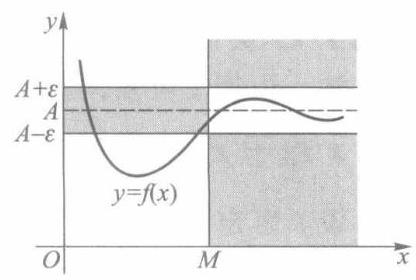
\includegraphics[width=.3\textwidth]{images/P007.jpg}
	\caption{图 $3-1$}
	\label{fig:P007}
\end{figure}

定义 1 的几何意义如图 3-1 所示,对任给的 \(\varepsilon  > 0\) ,在坐标平面上平行于 \(x\) 轴的两条直线 \(y = A + \varepsilon\) 与 \(y = A - \varepsilon\) , 围成以直线 \(y = A\) 为中心线、宽为 \({2\varepsilon }\) 的带形区域；定义中的 “当 \(x > M\) 时,有 \(\left| {f\left( x\right)  - A}\right|  < \varepsilon\) ” 表示: 在直线 \(x = M\) 的右方,曲线 \(y = f\left( x\right)\) 全部落在这个带形区域之内. 如果正数 \(\varepsilon\) 给得小一点,即当带形区域更窄一点时,直线 \(x = M\) 一般要往右平移; 但无论带形区域如何窄,总存在这样的正数 \(M\) , 使得曲线 \(y = f\left( x\right)\) 在直线 \(x = M\) 的右边部分全部落在这更窄的带形区域内.

现设 \(f\) 为定义在 \(U\left( {-\infty }\right)\) 或 \(U\left( \infty \right)\) 上的函数,当 \(x \rightarrow   - \infty\) 或 \(x \rightarrow  \infty\) 时,若函数值 \(f\left( x\right)\) 能无限地接近某定数 \(A\) ,则称 \(f\) 当 \(x \rightarrow   - \infty\) 或 \(x \rightarrow  \infty\) 时以 \(A\) 为极限,分别记作
\[
\mathop{\lim }\limits_{{x \rightarrow   - \infty }}f\left( x\right)  = A\text{ 或 }f\left( x\right)  \rightarrow  A\left( {x \rightarrow   - \infty }\right) \text{ ; }
\]
\[
\mathop{\lim }\limits_{{x \rightarrow  \infty }}f\left( x\right)  = A\text{ 或 }f\left( x\right)  \rightarrow  A\left( {x \rightarrow  \infty }\right) .
\]
这两种函数极限的精确定义与定义 1 相仿,只需把定义 1 中的 “ \(x > M\) ” 分别改为 “ \(x <  - M\) ” 或 “ \(\left| x\right|  > M\) ” 即可.

读者不难证明: 若 \(f\) 为定义在 \(U\left( \infty \right)\) 上的函数,则
\[
\mathop{\lim }\limits_{{x \rightarrow  \infty }}f\left( x\right)  = A \Leftrightarrow  \mathop{\lim }\limits_{{x \rightarrow   + \infty }}f\left( x\right)  = \mathop{\lim }\limits_{{x \rightarrow   - \infty }}f\left( x\right)  = A. \tag{1}
\]
%例 1
\begin{example}
证明 \(\mathop{\lim }\limits_{{x \rightarrow  \infty }}\frac{1}{x} = 0\) .
\end{example}


%证
\begin{proof}
任给 \(\varepsilon  > 0\) ,取 \(M = \frac{1}{\varepsilon }\) ,则当 \(\left| x\right|  > M\) 时,有
\[
\left| {\frac{1}{x} - 0}\right|  = \frac{1}{\left| x\right| } < \frac{1}{M} = \varepsilon ,
\]
所以 \(\mathop{\lim }\limits_{{x \rightarrow  \infty }}\frac{1}{x} = 0\) .
\end{proof}


%例 2
\begin{example}
证明: 1) \(\mathop{\lim }\limits_{{x \rightarrow   - \infty }}\arctan x =  - \frac{\pi }{2};2)\mathop{\lim }\limits_{{x \rightarrow   + \infty }}\arctan x = \frac{\pi }{2}\) .
\end{example}

%证
\begin{proof}
任给 \(\varepsilon  > 0\) ,由于
\[
\left| {\arctan x - \left( {-\frac{\pi }{2}}\right) }\right|  < \varepsilon  \tag{2}
\]
等价于 \(- \varepsilon  - \frac{\pi }{2} < \arctan x < \varepsilon  - \frac{\pi }{2}\) ,而此不等式的左半部分对任何 \(x\) 都成立,所以只需考察其右半部分 \(x\) 的变化范围. 为此,先限制 \(\varepsilon  < \frac{\pi }{2}\) ,则有
\[
x < \tan \left( {\varepsilon  - \frac{\pi }{2}}\right)  =  - \tan \left( {\frac{\pi }{2} - \varepsilon }\right) .
\]
故对任给的正数 \(\varepsilon \left( { < \frac{\pi }{2}}\right)\) ,只需取 \(M = \tan \left( {\frac{\pi }{2} - \varepsilon }\right)\) ,则当 \(x <  - M\) 时,便有 (2) 式成立. 这就证明了 1 ). 类似地可证 2 ).
\end{proof}


%注
\begin{remark}
由例 2 可知,当 \(x \rightarrow  \infty\) 时 \(\arctan x\) 不存在极限.
\end{remark}


\subsection{\(x\) 趋于 \({x}_{0}\) 时函数的极限}

设 \(f\) 为定义在点 \({x}_{0}\) 的某个空心邻域 \({U}^{ \circ  }\left( {x}_{0}\right)\) 上的函数. 现在讨论当 \(x\) 趋于 \({x}_{0}\left( {x \neq  {x}_{0}}\right)\) 时,对应的函数值能否趋于某个定数 \(A\) . 这类函数极限的精确定义如下.

%定义  2
\begin{definition}{函数极限的 \(\varepsilon  - \delta\) 定义}{def:函数极限的varepsilon-delta定义}
设函数 \(f\) 在点 \({x}_{0}\) 的某个空心邻域 \({U}^{ \circ  }\left( {{x}_{0};{\delta }^{\prime }}\right)\) 内有定义, \(A\) 为定数. 若对任给的 \(\varepsilon  > 0\) ,存在正数 \(\delta \left( { < {\delta }^{\prime }}\right)\) ,使得当 \(0 < \left| {x - {x}_{0}}\right|  < \delta\) 时,有
\[
\left| {f\left( x\right)  - A}\right|  < \varepsilon ,
\]
则称函数 \(f\) 当 \(x\) 趋于 \({x}_{0}\) 时以 \(A\) 为极限,记作
\[
\mathop{\lim }\limits_{{x \rightarrow  {x}_{0}}}f\left( x\right)  = A\text{ 或 }f\left( x\right)  \rightarrow  A\left( {x \rightarrow  {x}_{0}}\right) .
\]
\end{definition}

下面我们举例说明如何应用 \(\varepsilon  - \delta\) 定义来验证这种类型的函数极限. 请读者特别注意以下各例中 \(\delta\) 的值是怎样确定的.

%例 3
\begin{example}

\end{example}
设 \(f\left( x\right)  = \frac{{x}^{2} - 4}{x - 2}\) ,证明 \(\mathop{\lim }\limits_{{x \rightarrow  2}}f\left( x\right)  = 4\) .

%证
\begin{proof}

\end{proof}
由于当 \(x \neq  2\) 时,
\[
\left| {f\left( x\right)  - 4}\right|  = \left| {\frac{{x}^{2} - 4}{x - 2} - 4}\right|  = \left| {x + 2 - 4}\right|  = \left| {x - 2}\right| ,
\]
故对给定的 \(\varepsilon  > 0\) ,只要取 \(\delta  = \varepsilon\) ,则当 \(0 < \left| {x - 2}\right|  < \delta\) 时,有 \(\left| {f\left( x\right)  - 4}\right|  < \varepsilon\) . 这就证明了 \(\mathop{\lim }\limits_{{x \rightarrow  2}}f\left( x\right)  = 4\) .

%例 4
\begin{example}

\end{example}
证明: 1) \(\mathop{\lim }\limits_{{x \rightarrow  {x}_{0}}}\sin x = \sin {x}_{0}\) ; 2) \(\mathop{\lim }\limits_{{x \rightarrow  {x}_{0}}}\cos x = \cos {x}_{0}\) .

%证
\begin{proof}

\end{proof}
先建立一个不等式: 当 \(0 < x < \frac{\pi }{2}\) 时,有
\[
\sin x < x < \tan x\text{ . } \tag{3}
\]
\begin{figure}
	\centering
	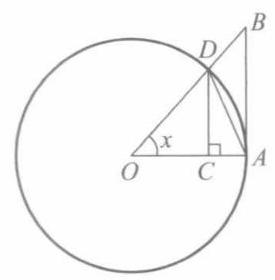
\includegraphics[width=.3\textwidth]{images/P008.jpg}
	\caption{图 $3-2$}
	\label{fig:P008}
\end{figure}

事实上,在如图 \(3-2\) 的单位圆内,当 \(0 < x < \frac{\pi }{2}\) 时,若用 \(S\) 表示面积, 显然有
\[
{S}_{\bigtriangleup {OAD}} < {S}_{\text{ 扇形 }{OAD}} < {S}_{\bigtriangleup {OAB}},
\]
即 \(\frac{1}{2}\sin x < \frac{1}{2}x < \frac{1}{2}\tan x\) ,由此立得 (3) 式.

又当 \(x \geq  \frac{\pi }{2}\) 时,有 \(\sin x \leq  1 < x\) ,故对一切 \(x > 0\) ,都有 \(\sin x < x\) ; 当 \(x < 0\) 时,由 \(\sin \left( {-x}\right)  <\)  \(- x\) 得 \(- \sin x <  - x\) . 综上,我们又得到不等式
\[
\left| {\sin x}\right|  \leq  \left| x\right| ,x \in  \mathbf{R}, \tag{4}
\]
其中等号仅当 \(x = 0\) 时成立.

现证 1). 由 (4) 式得
\[
\left| {\sin x - \sin {x}_{0}}\right|  = 2\left| {\cos \frac{x + {x}_{0}}{2}}\right| \left| {\sin \frac{x - {x}_{0}}{2}}\right|  \leq  \left| {x - {x}_{0}}\right| .
\]
对任给的 \(\varepsilon  > 0\) ,只要取 \(\delta  = \varepsilon\) ,则当 \(0 < \left| {x - {x}_{0}}\right|  < \delta\) 时,就有
\[
\left| {\sin x - \sin {x}_{0}}\right|  < \varepsilon .
\]
所以 \(\mathop{\lim }\limits_{{x \rightarrow  {x}_{0}}}\sin x = \sin {x}_{0}\) . 2) 的证明留给读者作为练习.

%例 5
\begin{example}

\end{example}
证明 \(\mathop{\lim }\limits_{{x \rightarrow  1}}\frac{{x}^{2} - 1}{2{x}^{2} - x - 1} = \frac{2}{3}\) .

%证
\begin{proof}

\end{proof}
当 \(x \neq  1\) 时,有
\[
\left| {\frac{{x}^{2} - 1}{2{x}^{2} - x - 1} - \frac{2}{3}}\right|  = \left| {\frac{x + 1}{{2x} + 1} - \frac{2}{3}}\right|  = \frac{\left| x - 1\right| }{3\left| {{2x} + 1}\right| }.
\]
若限制 \(x\) 于 \(0 < \left| {x - 1}\right|  < 1\) (此时 \(x > 0\) ),则 \(\left| {{2x} + 1}\right|  > 1\) . 于是,对任给的 \(\varepsilon  > 0\) ,只要取 \(\delta  = \min \{ {3\varepsilon },1\}\) ,则当 \(0 < \left| {x - 1}\right|  < \delta\) 时,便有
\[
\left| {\frac{{x}^{2} - 1}{2{x}^{2} - x - 1} - \frac{2}{3}}\right|  < \frac{\left| x - 1\right| }{3} < \varepsilon .
\]
%例 6
\begin{example}

\end{example}
证明 \(\mathop{\lim }\limits_{{x \rightarrow  {x}_{0}}}\sqrt{1 - {x}^{2}} = \sqrt{1 - {x}_{0}^{2}}\left( {\left| {x}_{0}\right|  < 1}\right)\) .

%证
\begin{proof}

\end{proof}
由于 \(\left| x\right|  \leq  1,\left| {x}_{0}\right|  < 1\) ,因此
\[
\left| {\sqrt{1 - {x}^{2}} - \sqrt{1 - {x}_{0}^{2}}}\right|  = \frac{\left| {x}_{0}^{2} - {x}^{2}\right| }{\sqrt{1 - {x}^{2}} + \sqrt{1 - {x}_{0}^{2}}}
\]
\[
\leq  \frac{\left| {x + {x}_{0}}\right| \left| {x - {x}_{0}}\right| }{\sqrt{1 - {x}_{0}^{2}}} \leq  \frac{2\left| {x - {x}_{0}}\right| }{\sqrt{1 - {x}_{0}^{2}}}.
\]
于是,对任给的 \(\varepsilon  > 0\) (不妨设 \(0 < \varepsilon  < 1\) ),取
\[
\delta  = \min \left\{  {\left| {{x}_{0} - 1}\right| ,\left| {{x}_{0} + 1}\right| ,\frac{\sqrt{1 - {x}_{0}^{2}}}{2}\varepsilon }\right\}  ,
\]
则当 \(0 < \left| {x - {x}_{0}}\right|  < \delta\) 时,就有 \(\left| {\sqrt{1 - {x}^{2}} - \sqrt{1 - {x}_{0}^{2}}}\right|  < \varepsilon\) .

应用 \(\varepsilon  - \delta\) 定义还立刻可得
\[
\mathop{\lim }\limits_{{x \rightarrow  {x}_{0}}}c = c,\mathop{\lim }\limits_{{x \rightarrow  {x}_{0}}}x = {x}_{0},
\]
这里 \(c\) 为常数, \({x}_{0}\) 为给定实数.

通过以上各个例子,读者对函数极限的 \(\varepsilon  - \delta\) 定义应能体会到下面几点:

1. 定义 2 中的正数 \(\delta\) ,相当于数列极限 \(\varepsilon  - N\) 定义中的 \(N\) ,它依赖于 \(\varepsilon\) ,但也不是由 \(\varepsilon\) 所唯一确定的.一般来说, \(\varepsilon\) 愈小, \(\delta\) 也相应地要小一些,而且把 \(\delta\) 取得更小些也无妨. 如在例 3 中可取 \(\delta  = \frac{\varepsilon }{2}\) 或 \(\delta  = \frac{\varepsilon }{3}\) ,等等.

2. 定义中只要求函数 \(f\) 在 \({x}_{0}\) 的某一空心邻域上有定义,而一般不考虑 \(f\) 在点 \({x}_{0}\) 处的函数值是否有定义,或者取什么值. 这是因为,对于函数极限我们所研究的是当 \(x\) 趋于 \({x}_{0}\) 过程中函数值的变化趋势. 如在例 3 中,函数 \(f\) 在点 \(x = 2\) 是没有定义的,但当 \(x \rightarrow  2\) 时 \(f\) 的函数值趋于一个定数.

3. 定义 2 中的不等式 \(0 < \left| {x - {x}_{0}}\right|  < \delta\) 等价于 \(x \in  {U}^{ \circ  }\left( {{x}_{0};\delta }\right)\) ,而不等式 \(\left| {f\left( x\right)  - A}\right|  < \varepsilon\) 等价于 \(f\left( x\right)  \in  U\left( {A;\varepsilon }\right)\) . 于是, \(\varepsilon  - \delta\) 定义又可写成

任给 \(\varepsilon  > 0\) ,存在 \(\delta  > 0\) ,使得对一切 \(x \in  {U}^{ \circ  }\left( {{x}_{0};\delta }\right)\) ,有 \(f\left( x\right)  \in  U\left( {A;\varepsilon }\right)\) .

或更简单地表述为

任给 \(\varepsilon  > 0\) ,存在 \(\delta  > 0\) ,使得 \(f\left( {{U}^{ \circ  }\left( {{x}_{0};\delta }\right) }\right)  \subset  U\left( {A;\varepsilon }\right)\) .

4. \(\varepsilon  - \delta\) 定义的几何意义如图 3-3 所示. 对任给的 \(\varepsilon  >\) 0,在坐标平面上画一条以直线 \(y = A\) 为中心线、宽为 \({2\varepsilon }\) 的横带,则必存在以直线 \(x = {x}_{0}\) 为中心线、宽为 \({2\delta }\) 的竖带,使函数 \(y = f\left( x\right)\) 的图像在该竖带中的部分全部落在横带内,但点 \(\left( {{x}_{0},f\left( {x}_{0}\right) }\right)\) 可能例外 (或无意义).

\begin{figure}
	\centering
	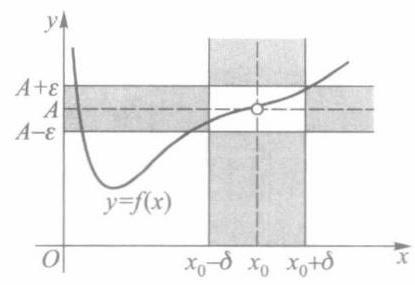
\includegraphics[width=.3\textwidth]{images/P009.jpg}
	\caption{图 $3-3$}
	\label{fig:P009}
\end{figure}

下面我们讨论单侧极限.

有些函数在其定义域上某些点左侧与右侧的解析式不同(如分段函数定义域上的某些点),或函数在某些点仅在其一侧有定义(如在定义区间端点处), 这时函数在那些点上的极限只能单侧地给出定义.

例如, 函数
\[
f\left( x\right)  = \left\{  \begin{array}{ll} {x}^{2}, & x \geq  0, \\  x, & x < 0 \end{array}\right.  \tag{5}
\]
当 \(x > 0\) 而趋于 0 时,应按 \(f\left( x\right)  = {x}^{2}\) 来考察函数值的变化趋势; 当 \(x < 0\) 而趋于 0 时,则应按 \(f\left( x\right)  = x\) 来考察. 又如函数 \(\sqrt{1 - {x}^{2}}\) 在其定义区间 \(\left\lbrack  {-1,1}\right\rbrack\) 端点 \(x =  \pm  1\) 处的极限,也只能在点 \(x =  - 1\) 的右侧和点 \(x = 1\) 的左侧来分别讨论.

%定义  3
\begin{definition}{单侧极限}{def:单侧极限}
设函数 \(f\) 在 \({U}_{ + }^{ \circ  }\left( {{x}_{0};{\delta }^{\prime }}\right)\) (或 \({U}_{ - }^{ \circ  }\left( {{x}_{0};{\delta }^{\prime }}\right)\) ) 上有定义, \(A\) 为定数. 若对任给的 \(\varepsilon  > 0\) ,存在正数 \(\delta \left( { < {\delta }^{\prime }}\right)\) ,使得当 \({x}_{0} < x < {x}_{0} + \delta\) (或 \({x}_{0} - \delta  < x < {x}_{0}\) ) 时,有
\[
\left| {f\left( x\right)  - A}\right|  < \varepsilon ,
\]
则称数 \(A\) 为函数 \(f\) 当 \(x\) 趋于 \({x}_{0}^{ + }\) (或 \({x}_{0}^{ - }\) ) 时的右 (左) 极限,记作
\[
\mathop{\lim }\limits_{{x \rightarrow  {x}_{0}^{ + }}}f\left( x\right)  = A\left( {\mathop{\lim }\limits_{{x \rightarrow  {x}_{0}^{ - }}}f\left( x\right)  = A}\right)
\]
或
\[
f\left( x\right)  \rightarrow  A\left( {x \rightarrow  {x}_{0}^{ + }}\right) \left( {f\left( x\right)  \rightarrow  A\left( {x \rightarrow  {x}_{0}^{ - }}\right) }\right) .
\]
右极限与左极限统称为单侧极限. \(f\) 在点 \({x}_{0}\) 的右极限与左极限又分别记为
\[
f\left( {{x}_{0} + 0}\right)  = \mathop{\lim }\limits_{{x \rightarrow  {x}_{0}^{ + }}}f\left( x\right) \text{ 与 }f\left( {{x}_{0} - 0}\right)  = \mathop{\lim }\limits_{{x \rightarrow  {x}_{0}^{ - }}}f\left( x\right) .
\]
\end{definition}

按定义 3 容易验证函数 (5) 在 \(x = 0\) 处的左、右极限分别为
\[
f\left( {0 - 0}\right)  = \mathop{\lim }\limits_{{x \rightarrow  {0}^{ - }}}f\left( x\right)  = \mathop{\lim }\limits_{{x \rightarrow  {0}^{ - }}}x = 0,
\]
\[
f\left( {0 + 0}\right)  = \mathop{\lim }\limits_{{x \rightarrow  {0}^{ + }}}f\left( x\right)  = \mathop{\lim }\limits_{{x \rightarrow  {0}^{ + }}}{x}^{2} = 0.
\]
同样还可验证符号函数 \(\operatorname{sgn}x\) 在 \(x = 0\) 处的左、右极限分别为
\[
\mathop{\lim }\limits_{{x \rightarrow  {0}^{ - }}}\operatorname{sgn}x = \mathop{\lim }\limits_{{x \rightarrow  {0}^{ - }}}\left( {-1}\right)  =  - 1,\mathop{\lim }\limits_{{x \rightarrow  {0}^{ + }}}\operatorname{sgn}x = \mathop{\lim }\limits_{{x \rightarrow  {0}^{ + }}}1 = 1.
\]
%例 7
\begin{example}

\end{example}
讨论函数 \(\sqrt{1 - {x}^{2}}\) 在定义区间端点 \(\pm  1\) 处的单侧极限.

%解
\begin{solution}

\end{solution}
由于 \(\left| x\right|  \leq  1\) ,故有
\[
1 - {x}^{2} = \left( {1 + x}\right) \left( {1 - x}\right)  \leq  2\left( {1 - x}\right) .
\]
任给 \(0 < \varepsilon  < 1\) ,当 \(2\left( {1 - x}\right)  < {\varepsilon }^{2}\) 时,就有
\[
\sqrt{1 - {x}^{2}} < \varepsilon \text{ . } \tag{6}
\]
于是取 \(\delta  = \frac{{\varepsilon }^{2}}{2}\) ,则当 \(0 < 1 - x < \delta\) 即 \(1 - \delta  < x < 1\) 时,(6) 式成立. 这就推出 \(\mathop{\lim }\limits_{{x \rightarrow  {1}^{ - }}}\sqrt{1 - {x}^{2}} = 0\) . 类似地可得 \(\mathop{\lim }\limits_{{x \rightarrow  {\left( -1\right) }^{ + }}}\sqrt{1 - {x}^{2}} = 0\) .

关于函数极限 \(\mathop{\lim }\limits_{{x \rightarrow  {x}_{0}}}f\left( x\right)\) 与相应的左、右极限之间的关系,有下述定理:

%定理 3.1
\begin{theorem}{}{the:}
\(\mathop{\lim }\limits_{{x \rightarrow  {x}_{0}}}f\left( x\right)  = A \Leftrightarrow  \mathop{\lim }\limits_{{x \rightarrow  {x}_{0}^{ + }}}f\left( x\right)  = \mathop{\lim }\limits_{{x \rightarrow  {x}_{0}^{ - }}}f\left( x\right)  = A\) .
\end{theorem}


这个定理的证明留给读者.

应用定理 3.1,除了可验证函数极限的存在 (如对函数 (3) 有 \(\mathop{\lim }\limits_{{x \rightarrow  0}}f\left( x\right)  = 0\) ),还常可说明某些函数极限的不存在,如前面提到的符号函数 \(\operatorname{sgn}x\) ,由于它在 \(x = 0\) 处的左、右极限不相等,所以 \(\mathop{\lim }\limits_{{x \rightarrow  0}}\operatorname{sgn}x\) 不存在.

\subsection{习题 3.1}

1. 按定义证明下列极限:

(1) \(\mathop{\lim }\limits_{{x \rightarrow   + \infty }}\frac{{6x} + 5}{x} = 6\) ;

(2) \(\mathop{\lim }\limits_{{x \rightarrow  2}}\left( {{x}^{2} - {6x} + {10}}\right)  = 2\) ;

(3) \(\mathop{\lim }\limits_{{x \rightarrow  \infty }}\frac{{x}^{2} - 5}{{x}^{2} - 1} = 1\) ;

(4) \(\mathop{\lim }\limits_{{x \rightarrow  {2}^{ - }}}\sqrt{4 - {x}^{2}} = 0\) ;

(5) \(\mathop{\lim }\limits_{{x \rightarrow  {x}_{0}}}\cos x = \cos {x}_{0}\) .

2. 根据定义 2 叙述 \(\mathop{\lim }\limits_{{x \rightarrow  {x}_{0}}}f\left( x\right)  \neq  A\) .

3. 设 \(\mathop{\lim }\limits_{{x \rightarrow  {x}_{0}}}f\left( x\right)  = A\) ,证明 \(\mathop{\lim }\limits_{{h \rightarrow  0}}f\left( {{x}_{0} + h}\right)  = A\) .

4. 证明: 若 \(\mathop{\lim }\limits_{{x \rightarrow  {x}_{0}}}f\left( x\right)  = A\) ,则 \(\mathop{\lim }\limits_{{x \rightarrow  {x}_{0}}}\left| {f\left( x\right) }\right|  = \left| A\right|\) . 当且仅当 \(A\) 为何值时反之也成立?

5. 证明定理 3.1 .

6. 讨论下列函数在 \(x \rightarrow  0\) 时的极限或左、右极限:

(1) \(f\left( x\right)  = \frac{\left| x\right| }{x}\) ;

(2) \(f\left( x\right)  = \left\lbrack  x\right\rbrack\) ;

(3) \(f\left( x\right)  = \left\{  \begin{array}{ll} {2}^{x}, & x > 0, \\  0, & x = 0, \\  1 + {x}^{2}, & x < 0. \end{array}\right.\)

7. 设 \(\mathop{\lim }\limits_{{x \rightarrow   + \infty }}f\left( x\right)  = A\) ,证明 \(\mathop{\lim }\limits_{{x \rightarrow  {0}^{ + }}}f\left( \frac{1}{x}\right)  = A\) .

8. 证明: 对黎曼函数 \(R\left( x\right)\) 有 \(\mathop{\lim }\limits_{{x \rightarrow  {x}_{0}}}R\left( x\right)  = 0,{x}_{0} \in  \left\lbrack  {0,1}\right\rbrack\) (当 \({x}_{0} = 0\) 或 1 时,考虑单侧极限).

\section{函数极限的性质}

在 §1 中我们引入了下述六种类型的函数极限:

1) \(\mathop{\lim }\limits_{{x \rightarrow   + \infty }}f\left( x\right)\) ; 2) \(\mathop{\lim }\limits_{{x \rightarrow   - \infty }}f\left( x\right)\) ; 3) \(\mathop{\lim }\limits_{{x \rightarrow  \infty }}f\left( x\right)\) ;

4) \(\mathop{\lim }\limits_{{x \rightarrow  {x}_{0}}}f\left( x\right)\) ; 5) \(\mathop{\lim }\limits_{{x \rightarrow  {x}_{0}^{ + }}}f\left( x\right)\) ; 6) \(\mathop{\lim }\limits_{{x \rightarrow  {x}_{0}^{ - }}}f\left( x\right)\) .

它们具有与数列极限相类似的一些性质, 下面以第 4 ) 种类型的极限为代表来叙述并证明这些性质. 至于其他类型极限的性质及其证明, 只要相应地做些修改即可.

%定理 3.2
\begin{theorem}{唯一性}{the:唯一性}
若极限 \(\mathop{\lim }\limits_{{x \rightarrow  {x}_{0}}}f\left( x\right)\) 存在,则此极限是唯一的.
\end{theorem}

%证
\begin{proof}
设 \(A,B\) 都是 \(f\) 当 \(x \rightarrow  {x}_{0}\) 时的极限,则对任给的 \(\varepsilon  > 0\) ,分别存在正数 \({\delta }_{1}\) 与 \({\delta }_{2}\) ,使得当 \(0 < \left| {x - {x}_{0}}\right|  < {\delta }_{1}\) 时,有
\[
\left| {f\left( x\right)  - A}\right|  < \varepsilon , \tag{1}
\]
当 \(0 < \left| {x - {x}_{0}}\right|  < {\delta }_{2}\) 时,有
\[
\left| {f\left( x\right)  - B}\right|  < \varepsilon . \tag{2}
\]
取 \(\delta  = \min \left( {{\delta }_{1},{\delta }_{2}}\right)\) ,则当 \(0 < \left| {x - {x}_{0}}\right|  < \delta\) 时,(1) 式与 (2) 式同时成立,故有
\[
\left| {A - B}\right|  = \left| {\left( {f\left( x\right)  - A}\right)  - \left( {f\left( x\right)  - B}\right) }\right|
\]
\[
\leq  \left| {f\left( x\right)  - A}\right|  + \left| {f\left( x\right)  - B}\right|  < {2\varepsilon }.
\]
由 \(\varepsilon\) 的任意性得 \(A = B\) . 这就证明了极限是唯一的.
\end{proof}


%定理 3.3
\begin{theorem}{局部有界性}{the:局部有界性}
若 \(\mathop{\lim }\limits_{{x \rightarrow  {x}_{0}}}f\left( x\right)\) 存在,则 \(f\) 在 \({x}_{0}\) 的某空心邻域 \({U}^{ \circ  }\left( {x}_{0}\right)\) 上有界.
\end{theorem}


%证
\begin{proof}
设 \(\mathop{\lim }\limits_{{x \rightarrow  {x}_{0}}}f\left( x\right)  = A\) . 取 \(\varepsilon  = 1\) ,则存在 \(\delta  > 0\) ,使得对一切 \(x \in  {U}^{ \circ  }\left( {{x}_{0};\delta }\right)\) ,有
\[
\left| {f\left( x\right)  - A}\right|  < 1 \Rightarrow  \left| {f\left( x\right) }\right|  < \left| A\right|  + 1.
\]
这就证明了 \(f\) 在 \({U}^{ \circ  }\left( {{x}_{0};\delta }\right)\) 上有界.
\end{proof}


%定理 3.4
\begin{theorem}{局部保号性}{the:局部保号性}
若 \(\mathop{\lim }\limits_{{x \rightarrow  {x}_{0}}}f\left( x\right)  = A > 0\) (或 \(< 0\) ),则对任何正数 \(r < A\) (或 \(r <  - A\) ), 存在 \({U}^{ \circ  }\left( {x}_{0}\right)\) ,使得对一切 \(x \in  {U}^{ \circ  }\left( {x}_{0}\right)\) ,有
\[
f\left( x\right)  > r > 0\left( {\text{ 或 }f\left( x\right)  <  - r < 0}\right) .
\]
\end{theorem}

%证
\begin{proof}
设 \(A > 0\) ,对任何 \(r \in  \left( {0,A}\right)\) ,取 \(\varepsilon  = A - r\) ,则存在 \(\delta  > 0\) ,使得对一切 \(x \in  {U}^{ \circ  }\left( {{x}_{0};\delta }\right)\) ,有
\[
f\left( x\right)  > A - \varepsilon  = r,
\]
这就证得结论. 对于 \(A < 0\) 的情形可类似地证明.
\end{proof}


%注
\begin{remark}
在以后应用局部保号性时,常取 \(r = \frac{A}{2}\) .
\end{remark}


%定理 3.5
\begin{theorem}{保不等式性}{the:保不等式性}
设 \(\mathop{\lim }\limits_{{x \rightarrow  {x}_{0}}}f\left( x\right)\) 与 \(\mathop{\lim }\limits_{{x \rightarrow  {x}_{0}}}g\left( x\right)\) 都存在,且在某邻域 \({U}^{ \circ  }\left( {{x}_{0};{\delta }^{\prime }}\right)\) 上有 \(f\left( x\right)  \leq  g\left( x\right)\) ,则
\[
\mathop{\lim }\limits_{{x \rightarrow  {x}_{0}}}f\left( x\right)  \leq  \mathop{\lim }\limits_{{x \rightarrow  {x}_{0}}}g\left( x\right) . \tag{3}
\]
\end{theorem}

%证
\begin{proof}
设 \(\mathop{\lim }\limits_{{x \rightarrow  {x}_{0}}}f\left( x\right)  = A,\mathop{\lim }\limits_{{x \rightarrow  {x}_{0}}}g\left( x\right)  = B\) ,则对任给的 \(\varepsilon  > 0\) ,分别存在正数 \({\delta }_{1}\) 与 \({\delta }_{2}\) ,使得当 \(0 < \left| {x - {x}_{0}}\right|  < {\delta }_{1}\) 时,有
\[
A - \varepsilon  < f\left( x\right) , \tag{4}
\]
当 \(0 < \left| {x - {x}_{0}}\right|  < {\delta }_{2}\) 时,有
\[
g\left( x\right)  < B + \varepsilon . \tag{5}
\]
令 \(\delta  = \min \left\{  {{\delta }^{\prime },{\delta }_{1},{\delta }_{2}}\right\}\) ,则当 \(0 < \left| {x - {x}_{0}}\right|  < \delta\) 时,不等式 \(f\left( x\right)  \leq  g\left( x\right)\) 与 (4)、(5) 两式同时成立, 于是有
\[
A - \varepsilon  < f\left( x\right)  \leq  g\left( x\right)  < B + \varepsilon ,
\]
从而 \(A < B + {2\varepsilon }\) . 由 \(\varepsilon\) 的任意性推出 \(A \leq  B\) ,即 (3) 式成立.
\end{proof}


%定理 3.6
\begin{theorem}{迫敛性}{the:迫敛性}
设 \(\mathop{\lim }\limits_{{x \rightarrow  {x}_{0}}}f\left( x\right)  = \mathop{\lim }\limits_{{x \rightarrow  {x}_{0}}}g\left( x\right)  = A\) ,且在某 \({U}^{ \circ  }\left( {{x}_{0};{\delta }^{\prime }}\right)\) 上有
\[
f\left( x\right)  \leq  h\left( x\right)  \leq  g\left( x\right) , \tag{6}
\]
则 \(\mathop{\lim }\limits_{{x \rightarrow  {x}_{0}}}h\left( x\right)  = A\) .
\end{theorem}

%证
\begin{proof}
按假设,对任给的 \(\varepsilon  > 0\) ,分别存在正数 \({\delta }_{1}\) 与 \({\delta }_{2}\) ,使得当 \(0 < \left| {x - {x}_{0}}\right|  < {\delta }_{1}\) 时,有
\[
A - \varepsilon  < f\left( x\right) , \tag{7}
\]
当 \(0 < \left| {x - {x}_{0}}\right|  < {\delta }_{2}\) 时,有
\[
g\left( x\right)  < A + \varepsilon . \tag{8}
\]
令 \(\delta  = \min \left\{  {{\delta }^{\prime },{\delta }_{1},{\delta }_{2}}\right\}\) ,则当 \(0 < \left| {x - {x}_{0}}\right|  < \delta\) 时,不等式 (6)、(7)、(8) 同时成立,故有
\[
A - \varepsilon  < f\left( x\right)  \leq  h\left( x\right)  \leq  g\left( x\right)  < A + \varepsilon ,
\]
由此得 \(\left| {h\left( x\right)  - A}\right|  < \varepsilon\) ,所以 \(\mathop{\lim }\limits_{{x \rightarrow  {x}_{0}}}h\left( x\right)  = A\) .
\end{proof}


%定理 3.7
\begin{theorem}{四则运算法则}{the:四则运算法则}
若极限 \(\mathop{\lim }\limits_{{x \rightarrow  {x}_{0}}}f\left( x\right)\) 与 \(\mathop{\lim }\limits_{{x \rightarrow  {x}_{0}}}g\left( x\right)\) 都存在,则函数 \(f \pm  g,f \cdot  g\) 当 \(x \rightarrow  {x}_{0}\) 时极限也存在,且

1) \(\mathop{\lim }\limits_{{x \rightarrow  {x}_{0}}}\left\lbrack  {f\left( x\right)  \pm  g\left( x\right) }\right\rbrack   = \mathop{\lim }\limits_{{x \rightarrow  {x}_{0}}}f\left( x\right)  \pm  \mathop{\lim }\limits_{{x \rightarrow  {x}_{0}}}g\left( x\right)\) ;

2) \(\mathop{\lim }\limits_{{x \rightarrow  {x}_{0}}}\left\lbrack  {f\left( x\right) g\left( x\right) }\right\rbrack   = \mathop{\lim }\limits_{{x \rightarrow  {x}_{0}}}f\left( x\right)  \cdot  \mathop{\lim }\limits_{{x \rightarrow  {x}_{0}}}g\left( x\right)\) ;

又若 \(\mathop{\lim }\limits_{{x \rightarrow  {x}_{0}}}g\left( x\right)  \neq  0\) ,则 \(f/g\) 当 \(x \rightarrow  {x}_{0}\) 时极限存在,且有

3) \(\mathop{\lim }\limits_{{x \rightarrow  {x}_{0}}}\frac{f\left( x\right) }{g\left( x\right) } = \mathop{\lim }\limits_{{x \rightarrow  {x}_{0}}}f\left( x\right) /\mathop{\lim }\limits_{{x \rightarrow  {x}_{0}}}g\left( x\right)\) .
\end{theorem}

这个定理的证明类似于数列极限中的相应定理, 留给读者作为练习.

利用函数极限的迫敛性与四则运算法则, 我们可从一些简单的函数极限出发, 计算较复杂的函数极限.

%例 1
\begin{example}
求 \(\mathop{\lim }\limits_{{x \rightarrow  0}}x\left\lbrack  \frac{1}{x}\right\rbrack\) .
\end{example}


%解
\begin{solution}
由第一章 §3 习题 12,当 \(x > 0\) 时,有
\[
1 - x < x\left\lbrack  \frac{1}{x}\right\rbrack   \leq  1,
\]
而 \(\mathop{\lim }\limits_{{x \rightarrow  {0}^{ + }}}\left( {1 - x}\right)  = 1\) ,故由迫敛性得
\[
\mathop{\lim }\limits_{{x \rightarrow  {0}^{ + }}}x\left\lbrack  \frac{1}{x}\right\rbrack   = 1.
\]
另一方面,当 \(x < 0\) 时,有 \(1 \leq  x\left\lbrack  \frac{1}{x}\right\rbrack   < 1 - x\) ,故由迫敛性又可得
\[
\mathop{\lim }\limits_{{x \rightarrow  {0}^{ - }}}x\left\lbrack  \frac{1}{x}\right\rbrack   = 1.
\]
综上,我们求得 \(\mathop{\lim }\limits_{{x \rightarrow  0}}x\left\lbrack  \frac{1}{x}\right\rbrack   = 1\) .
\end{solution}


%例 2
\begin{example}
求 \(\mathop{\lim }\limits_{{x \rightarrow  \frac{\pi }{4}}}\left( {x\tan x - 1}\right)\) .
\end{example}


%解
\begin{solution}
由 \(x\tan x = x\frac{\sin x}{\cos x}\) 及 §1 例 4 所得的
\[
\mathop{\lim }\limits_{{x \rightarrow  \frac{\pi }{4}}}\sin x = \sin \frac{\pi }{4} = \frac{\sqrt{2}}{2} = \mathop{\lim }\limits_{{x \rightarrow  \frac{\pi }{4}}}\cos x,
\]
并按四则运算法则有
\[
\mathop{\lim }\limits_{{x \rightarrow  \frac{\pi }{4}}}\left( {x\tan x - 1}\right)  = \mathop{\lim }\limits_{{x \rightarrow  \frac{\pi }{4}}}x \cdot  \frac{\mathop{\lim }\limits_{{x \rightarrow  \frac{\pi }{4}}}\sin x}{\mathop{\operatorname{limcos}}\limits_{{x \rightarrow  \frac{\pi }{4}}}x} - \mathop{\lim }\limits_{{x \rightarrow  \frac{\pi }{4}}}1 = \frac{\pi }{4} - 1.
\]
\end{solution}

%例 3
\begin{example}
求极限 \(\mathop{\lim }\limits_{{x \rightarrow  1}}\frac{1 + x + \cdots  + {x}^{n} - n - 1}{x - 1}\) .
\end{example}


%解
\begin{solution}
对任意正整数 \(k\) ,当 \(x \neq  1\) 时,有
\[
\frac{{x}^{k} - 1}{x - 1} = \frac{\left( {x - 1}\right) \left( {1 + x + \cdots  + {x}^{k - 1}}\right) }{x - 1} = 1 + x + \cdots  + {x}^{k - 1},
\]
故
\[
\mathop{\lim }\limits_{{x \rightarrow  1}}\frac{1 + x + \cdots  + {x}^{n} - n - 1}{x - 1} = \mathop{\lim }\limits_{{x \rightarrow  1}}\mathop{\sum }\limits_{{k = 1}}^{n}\frac{{x}^{k} - 1}{x - 1}
\]
\[
= \mathop{\sum }\limits_{{k = 1}}^{n}\mathop{\lim }\limits_{{x \rightarrow  1}}\left( {1 + x + \cdots  + {x}^{k - 1}}\right)  = \mathop{\sum }\limits_{{k = 1}}^{n}k = \frac{n\left( {n + 1}\right) }{2}.
\]
\end{solution}

%例 4
\begin{example}
证明 \(\mathop{\lim }\limits_{{x \rightarrow  0}}{a}^{x} = 1\left( {a > 1}\right)\) .
\end{example}


%证
\begin{proof}
任给 \(\varepsilon  > 0\) ,因为 \(\mathop{\lim }\limits_{{n \rightarrow  \infty }}{a}^{\frac{1}{n}} = 1,\mathop{\lim }\limits_{{n \rightarrow  \infty }}{a}^{-\frac{1}{n}} = 1\) ,所以存在 \(N\) ,使得
\[
{a}^{\frac{1}{N}} - 1 < \varepsilon ,\;1 - {a}^{-\frac{1}{N}} < \varepsilon .
\]
取 \(\delta  = \frac{1}{N}\) ,当 \(0 < \left| x\right|  < \delta\) 时,
\[
- \varepsilon  < {a}^{-\frac{1}{N}} - 1 < {a}^{x} - 1 < {a}^{\frac{1}{N}} - 1 < \varepsilon ,
\]
即 \(\left| {{a}^{x} - 1}\right|  < \varepsilon\) ,从而 \(\mathop{\lim }\limits_{{x \rightarrow  0}}{a}^{x} = 1\) .
\end{proof}


\subsection{习题 3.2}

1. 求下列极限:

(1) \(\lim 2\left( {\sin x - \cos x - {x}^{2}}\right)\) ;

(2) \(\mathop{\lim }\limits_{{x \rightarrow  0}}\frac{{x}^{2} - 1}{2{x}^{2} - x - 1}\) ; \(x \rightarrow  \frac{\pi }{2}\)

(3) \(\mathop{\lim }\limits_{{x \rightarrow  1}}\frac{{x}^{2} - 1}{2{x}^{2} - x - 1}\) ;

(4) \(\mathop{\lim }\limits_{{x \rightarrow  0}}\frac{{\left( x - 1\right) }^{3} + \left( {1 - {3x}}\right) }{{x}^{2} + 2{x}^{3}}\) ;

(5) \(\mathop{\lim }\limits_{{x \rightarrow  1}}\frac{{x}^{n} - 1}{{x}^{m} - 1}\left( {n,m\text{ 为正整数 }}\right)\) ;

(6) \(\mathop{\lim }\limits_{{x \rightarrow  4}}\frac{\sqrt{1 + {2x}} - 3}{\sqrt{x} - 2}\) ;

(7) \(\mathop{\lim }\limits_{{x \rightarrow  0}}\frac{\sqrt{{a}^{2} + x} - a}{x}\left( {a > 0}\right)\) ;

(8) \(\mathop{\lim }\limits_{{x \rightarrow   + \infty }}\frac{{\left( 3x + 6\right) }^{70}{\left( 8x - 5\right) }^{20}}{{\left( 5x - 1\right) }^{90}}\) .

2. 利用迫敛性求极限:

(1) \(\mathop{\lim }\limits_{{x \rightarrow   - \infty }}\frac{x - \cos x}{x}\) ;

(2) \(\mathop{\lim }\limits_{{x \rightarrow   + \infty }}\frac{x\sin x}{{x}^{2} - 4}\) .

3. 设 \(\mathop{\lim }\limits_{{x \rightarrow  {x}_{0}}}f\left( x\right)  = A,\mathop{\lim }\limits_{{x \rightarrow  {x}_{0}}}g\left( x\right)  = B\) . 证明:

(1) \(\mathop{\lim }\limits_{{x \rightarrow  {x}_{0}}}\left\lbrack  {f\left( x\right)  \pm  g\left( x\right) }\right\rbrack   = A \pm  B\) ;

(2) \(\mathop{\lim }\limits_{{x \rightarrow  {x}_{0}}}\left\lbrack  {f\left( x\right) g\left( x\right) }\right\rbrack   = {AB}\) ;

(3) \(\mathop{\lim }\limits_{{x \rightarrow  {x}_{0}}}\frac{f\left( x\right) }{g\left( x\right) } = \frac{A}{B}\) (当 \(B \neq  0\) 时).

4. 设
\[
f\left( x\right)  = \frac{{a}_{0}{x}^{m} + {a}_{1}{x}^{m - 1} + \cdots  + {a}_{m - 1}x + {a}_{m}}{{b}_{0}{x}^{n} + {b}_{1}{x}^{n - 1} + \cdots  + {b}_{n - 1}x + {b}_{n}},{a}_{0} \neq  0,{b}_{0} \neq  0,m \leq  n,
\]
试求 \(\mathop{\lim }\limits_{{x \rightarrow   + \infty }}f\left( x\right)\) .

5. 设 \(f\left( x\right)  > 0,\mathop{\lim }\limits_{{x \rightarrow  {x}_{0}}}f\left( x\right)  = A\) . 证明
\[
\mathop{\lim }\limits_{{x \rightarrow  {x}_{0}}}\sqrt[n]{f\left( x\right) } = \sqrt[n]{A},
\]
其中 \(n \geq  2\) 为正整数.



6. 证明 \(\mathop{\lim }\limits_{{x \rightarrow  0}}{a}^{x} = 1\left( {0 < a < 1}\right)\) .

7. 设 \(\mathop{\lim }\limits_{{x \rightarrow  {x}_{0}}}f\left( x\right)  = A,\mathop{\lim }\limits_{{x \rightarrow  {x}_{0}}}g\left( x\right)  = B\) .

(1) 若在某 \({U}^{ \circ  }\left( {x}_{0}\right)\) 上有 \(f\left( x\right)  < g\left( x\right)\) ,问是否必有 \(A < B\) ？为什么？

(2)证明: 若 \(A > B\) ,则在某 \({U}^{ \circ  }\left( {x}_{0}\right)\) 上有 \(f\left( x\right)  > g\left( x\right)\) .

8. 求下列极限 (其中 \(n\) 皆为正整数):

(1) \(\mathop{\lim }\limits_{{x \rightarrow  {0}^{ - }}}\frac{\left| x\right| }{x}\frac{1}{1 + {x}^{n}}\) ;

(2) \(\mathop{\lim }\limits_{{x \rightarrow  {0}^{ + }}}\frac{\left| x\right| }{x}\frac{1}{1 + {x}^{n}}\) ;

(3) \(\mathop{\lim }\limits_{{x \rightarrow   - 1}}\left( {\frac{1}{x + 1} - \frac{3}{{x}^{3} + 1}}\right)\) ;

(4) \(\mathop{\lim }\limits_{{x \rightarrow  0}}\frac{\sqrt[n]{1 + x} - 1}{x}\) ;

(5) \(\mathop{\lim }\limits_{{x \rightarrow  \infty }}\frac{\left\lbrack  x\right\rbrack  }{x}\) (提示: 参照例 1).

9. (1) 证明: 若 \(\mathop{\lim }\limits_{{x \rightarrow  0}}f\left( {x}^{3}\right)\) 存在,则 \(\mathop{\lim }\limits_{{x \rightarrow  0}}f\left( x\right)  = \mathop{\lim }\limits_{{x \rightarrow  0}}f\left( {x}^{3}\right)\) .

(2) 若 \(\mathop{\lim }\limits_{{x \rightarrow  0}}f\left( {x}^{2}\right)\) 存在,试问是否成立 \(\mathop{\lim }\limits_{{x \rightarrow  0}}f\left( x\right)  = \mathop{\lim }\limits_{{x \rightarrow  0}}f\left( {x}^{2}\right)\) ?

\section{函数极限存在的条件}

与讨论数列极限存在的条件一样, 我们将从函数值的变化趋势来判断其极限的存在性. 下面的定理只对 \(x \rightarrow  {x}_{0}\) 这种类型的函数极限进行论述,但其结论对其他类型的函数极限也是成立的. 下述归结原则有时称为海涅 (Heine) 定理.

%定理 3.8
\begin{theorem}{归结原则}{the:归结原则}
设 \(f\) 在 \({U}^{ \circ  }\left( {{x}_{0};{\delta }^{\prime }}\right)\) 上有定义. \(\mathop{\lim }\limits_{{x \rightarrow  {x}_{0}}}f\left( x\right)\) 存在的充要条件是: 对任何含于 \({U}^{ \circ  }\left( {{x}_{0};{\delta }^{\prime }}\right)\) 且以 \({x}_{0}\) 为极限的数列 \(\left\{  {x}_{n}\right\}\) ,极限 \(\mathop{\lim }\limits_{{n \rightarrow  \infty }}f\left( {x}_{n}\right)\) 都存在且相等.
\end{theorem}

%证
\begin{proof}
必要性 设 \(\mathop{\lim }\limits_{{x \rightarrow  {x}_{0}}}f\left( x\right)  = A\) ,则对任给的 \(\varepsilon  > 0\) ,存在正数 \(\delta \left( { \leq  {\delta }^{\prime }}\right)\) ,使得当 \(0 < \left| {x - {x}_{0}}\right|  < \delta\) 时,有 \(\left| {f\left( x\right)  - A}\right|  < \varepsilon\) .

另一方面,设数列 \(\left\{  {x}_{n}\right\}   \subset  {U}^{ \circ  }\left( {{x}_{0};{\delta }^{\prime }}\right)\) 且 \(\mathop{\lim }\limits_{{n \rightarrow  \infty }}{x}_{n} = {x}_{0}\) ,则对上述的 \(\delta  > 0\) ,存在 \(N > 0\) ,使得当 \(n > N\) 时,有 \(0 < \left| {{x}_{n} - {x}_{0}}\right|  < \delta\) ,从而有 \(\left| {f\left( {x}_{n}\right)  - A}\right|  < \varepsilon\) . 这就证明了 \(\mathop{\lim }\limits_{{n \rightarrow  \infty }}f\left( {x}_{n}\right)  = A\) .

充分性 设对任何数列 \(\left\{  {x}_{n}\right\}   \subset  {U}^{ \circ  }\left( {{x}_{0};{\delta }^{\prime }}\right)\) 且 \(\mathop{\lim }\limits_{{n \rightarrow  \infty }}{x}_{n} = {x}_{0}\) ,有 \(\mathop{\lim }\limits_{{n \rightarrow  \infty }}f\left( {x}_{n}\right)  = A\) ,则可用反证法推出 \(\mathop{\lim }\limits_{{x \rightarrow  {x}_{0}}}f\left( x\right)  = A\) . 事实上,倘若当 \(x \rightarrow  {x}_{0}\) 时 \(f\) 不以 \(A\) 为极限,则存在某 \({\varepsilon }_{0} > 0\) ,对任何 \(\delta  > 0\) (不论多么小),总存在一点 \(x\) ,尽管 \(0 < \left| {x - {x}_{0}}\right|  < \delta\) ,但有 \(\left| {f\left( x\right)  - A}\right|  \geq  {\varepsilon }_{0}\) (§ 1 习题 2). 现依次取 \(\delta  = {\delta }^{\prime },\frac{{\delta }^{\prime }}{2},\frac{{\delta }^{\prime }}{3},\cdots ,\frac{{\delta }^{\prime }}{n},\cdots\) ,则存在相应的点 \({x}_{1},{x}_{2},{x}_{3},\cdots ,{x}_{n},\cdots\) ,使得
\[
0 < \left| {{x}_{n} - {x}_{0}}\right|  < \frac{{\delta }^{\prime }}{n}\text{ ,而 }\left| {f\left( {x}_{n}\right)  - A}\right|  \geq  {\varepsilon }_{0},n = 1,2,\cdots \text{ . }
\]
显然数列 \(\left\{  {x}_{n}\right\}   \subset  {U}^{ \circ  }\left( {{x}_{0};{\delta }^{\prime }}\right)\) 且 \(\mathop{\lim }\limits_{{n \rightarrow  \infty }}{x}_{n} = {x}_{0}\) ,但当 \(n \rightarrow  \infty\) 时 \(f\left( {x}_{n}\right)\) 不趋于 \(A\) . 这与假设相矛盾, 所以必有 \(\mathop{\lim }\limits_{{x \rightarrow  {x}_{0}}}f\left( x\right)  = A\) .
\end{proof}


%注
\begin{remark}
1 归结原则也可简述为:
\[
\mathop{\lim }\limits_{{x \rightarrow  {x}_{0}}}f\left( x\right)  = A \Leftrightarrow  \text{ 对任何 }{x}_{n} \rightarrow  {x}_{0}\left( {n \rightarrow  \infty }\right) \text{ 有 }\mathop{\lim }\limits_{{n \rightarrow  \infty }}f\left( {x}_{n}\right)  = A\text{ . }
\]
\end{remark}

%注
\begin{remark}
2 若可找到一个以 \({x}_{0}\) 为极限的数列 \(\left\{  {x}_{n}\right\}\) ,使 \(\mathop{\lim }\limits_{{n \rightarrow  \infty }}f\left( {x}_{n}\right)\) 不存在,或找到两个都以 \({x}_{0}\) 为极限的数列 \(\left\{  {x}_{n}^{\prime }\right\}\) 与 \(\left\{  {x}_{n}^{\prime \prime }\right\}\) ,使 \(\mathop{\lim }\limits_{{n \rightarrow  \infty }}f\left( {x}_{n}^{\prime }\right)\) 与 \(\mathop{\lim }\limits_{{n \rightarrow  \infty }}f\left( {x}_{n}^{\prime \prime }\right)\) 都存在而不相等,则 \(\mathop{\lim }\limits_{{x \rightarrow  {x}_{0}}}f\left( x\right)\) 不存在.
\end{remark}


%例 1
\begin{example}
证明极限 \(\mathop{\lim }\limits_{{x \rightarrow  0}}\sin \frac{1}{x}\) 不存在.
\end{example}


%证
\begin{proof}
设 \({x}_{n}^{\prime } = \frac{1}{n\pi },{x}_{n}^{\prime \prime } = \frac{1}{{2n\pi } + \frac{\pi }{2}}\left( {n = 1,2,\cdots }\right)\) ,则显然有
\[
{x}_{n}^{\prime } \rightarrow  0,{x}_{n}^{\prime \prime } \rightarrow  0\left( {n \rightarrow  \infty }\right) ,
\]
\[
\sin \frac{1}{{x}_{n}^{\prime }} = 0 \rightarrow  0,\sin \frac{1}{{x}_{n}^{\prime \prime }} = 1 \rightarrow  1\left( {n \rightarrow  \infty }\right) .
\]
故由归结原则即得结论.

\end{proof}




\begin{figure}
    \centering
    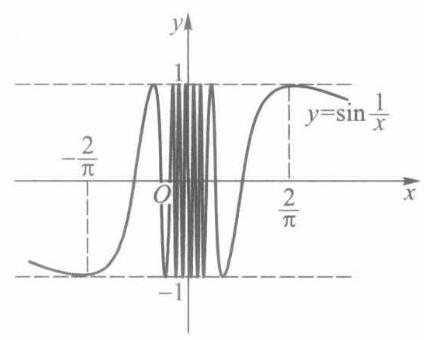
\includegraphics[width=.3\textwidth]{images/P010.jpg}
    \caption{图 $3-4$}
    \label{fig:P010}
\end{figure}

函数 \(y = \sin \frac{1}{x}\) 的图像如图 \(3-4\) 所示. 由图像可见, 当 \(x \rightarrow  0\) 时,其函数值无限次地在 \(-1\) 与 1 的范围内振荡,而不趋于任何确定的数.

归结原则的意义在于把函数极限归结为数列极限问题来处理. 从而, 我们能应用归结原则和数列极限的有关性质来证明上一节中所述的函数极限的所有性质.

对于 \(x \rightarrow  {x}_{0}^{ + },x \rightarrow  {x}_{0}^{ - },x \rightarrow   + \infty\) 和 \(x \rightarrow   - \infty\) 这四种类型的单侧极限,相应的归结原则可表示为更强的形式. 现以 \(x \rightarrow  {x}_{0}^{ + }\) 这种类型为例阐述如下:

%定理 3.9
\begin{theorem}{单侧极限}{the:单侧极限}
设函数 \(f\) 在点 \({x}_{0}\) 的某空心右邻域 \({U}_{ + }^{ \circ  }\left( {x}_{0}\right)\) 有定义. \(\mathop{\lim }\limits_{{x \rightarrow  {x}_{0}^{ + }}}f\left( x\right)  = A\) 的充要条件是: 对任何以 \({x}_{0}\) 为极限的递减数列 \(\left\{  {x}_{n}\right\}   \subset  {U}_{ + }^{ \circ  }\left( {x}_{0}\right)\) ,有 \(\mathop{\lim }\limits_{{n \rightarrow  \infty }}f\left( {x}_{n}\right)  = A\) .
\end{theorem}


这个定理的证明可仿照定理 3.8 进行,但在运用反证法证明充分性时,对 \(\delta\) 的取法要作适当的修改,以保证所找到的数列 \(\left\{  {x}_{n}\right\}\) 能递减地趋于 \({x}_{0}\) . 证明的细节留给读者作为练习.

相应于数列极限的单调有界定理, 关于上述四类单侧极限也有相应的定理. 现以 \(x \rightarrow  {x}_{0}^{ + }\) 这种类型为例叙述如下.

%定理 3.10
\begin{theorem}{右极限存在}{the:右极限存在}
设 \(f\) 为定义在 \({U}_{ + }^{ \circ  }\left( {x}_{0}\right)\) 上的单调有界函数,则右极限 \(\mathop{\lim }\limits_{{x \rightarrow  {x}_{0}^{ + }}}f\left( x\right)\) 存在.
\end{theorem}


%证
\begin{proof}
不妨设 \(f\) 在 \({U}_{ + }^{ \circ  }\left( {x}_{0}\right)\) 上递增. 因 \(f\) 在 \({U}_{ + }^{ \circ  }\left( {x}_{0}\right)\) 上有界,由确界原理, \(\mathop{\inf }\limits_{{x \in  {U}_{ + }^{ \circ  }\left( {x}_{0}\right) }}f\left( x\right)\) 存在,记为 \(A\) . 下证 \(\mathop{\lim }\limits_{{x \rightarrow  {x}_{0}^{ + }}}f\left( x\right)  = A\) .

事实上,任给 \(\varepsilon  > 0\) ,按下确界定义,存在 \({x}^{\prime } \in  {U}_{ + }^{ \circ  }\left( {x}_{0}\right)\) ,使得 \(f\left( {x}^{\prime }\right)  < A + \varepsilon\) . 取 \(\delta  = {x}^{\prime } - {x}_{0} >\) 0,则由 \(f\) 的递增性,对一切 \(x \in  \left( {{x}_{0},{x}^{\prime }}\right)  = {U}_{ + }^{ \circ  }\left( {{x}_{0};\delta }\right)\) ,有
\[
f\left( x\right)  \leq  f\left( {x}^{\prime }\right)  < A + \varepsilon .
\]
另一方面,由 \(A \leq  f\left( x\right)\) ,更有 \(A - \varepsilon  < f\left( x\right)\) . 从而对一切 \(x \in  {U}_{ + }^{ \circ  }\left( {{x}_{0};\delta }\right)\) ,有
\[
A - \varepsilon  < f\left( x\right)  < A + \varepsilon ,
\]
这就证得 \(\mathop{\lim }\limits_{{x \rightarrow  {x}_{0}^{ + }}}f\left( x\right)  = A\) .
\end{proof}


最后, 我们叙述并证明关于函数极限的柯西准则.

%定理 3.11
\begin{theorem}{柯西准则}{the:柯西准则}
设函数 \(f\) 在 \({U}^{ \circ  }\left( {{x}_{0};{\delta }^{\prime }}\right)\) 上有定义. \(\mathop{\lim }\limits_{{x \rightarrow  {x}_{0}}}f\left( x\right)\) 存在的充要条件是:任给 \(\varepsilon  > 0\) ,存在正数 \(\delta \left( { < {\delta }^{\prime }}\right)\) ,使得对任何 \({x}^{\prime },{x}^{\prime \prime } \in  {U}^{ \circ  }\left( {{x}_{0};\delta }\right)\) ,有 \(\left| {f\left( {x}^{\prime }\right)  - f\left( {x}^{\prime \prime }\right) }\right|  < \varepsilon\) .
\end{theorem}

%证
\begin{proof}
必要性 设 \(\mathop{\lim }\limits_{{x \rightarrow  {x}_{0}}}f\left( x\right)  = A\) ,则对任给的 \(\varepsilon  > 0\) ,存在正数 \(\delta \left( { < {\delta }^{\prime }}\right)\) ,使得对任何 \(x \in  {U}^{ \circ  }\left( {{x}_{0};\delta }\right)\) ,有 \(\left| {f\left( x\right)  - A}\right|  < \frac{\varepsilon }{2}\) . 于是对任何 \({x}^{\prime },{x}^{\prime \prime } \in  {U}^{ \circ  }\left( {{x}_{0};\delta }\right)\) ,有
\[
\left| {f\left( {x}^{\prime }\right)  - f\left( {x}^{\prime \prime }\right) }\right|  \leq  \left| {f\left( {x}^{\prime }\right)  - A}\right|  + \left| {f\left( {x}^{\prime \prime }\right)  - A}\right|  < \frac{\varepsilon }{2} + \frac{\varepsilon }{2} = \varepsilon .
\]
充分性 设数列 \(\left\{  {x}_{n}\right\}   \subset  {U}^{ \circ  }\left( {{x}_{0};\delta }\right)\) 且 \(\mathop{\lim }\limits_{{n \rightarrow  \infty }}{x}_{n} = {x}_{0}\) . 按假设,对任给的 \(\varepsilon  > 0\) ,存在正数 \(\delta \left( { < {\delta }^{\prime }}\right)\) ,使得对任何 \({x}^{\prime },{x}^{\prime \prime } \in  {U}^{ \circ  }\left( {{x}_{0};\delta }\right)\) ,有 \(\left| {f\left( {x}^{\prime }\right)  - f\left( {x}^{\prime \prime }\right) }\right|  < \varepsilon\) . 由于 \({x}_{n} \rightarrow  {x}_{0}\left( {n \rightarrow  \infty }\right)\) ,对上述的 \(\delta  > 0\) ,存在 \(N > 0\) ,使得当 \(n,m > N\) 时,有 \({x}_{n},{x}_{m} \in  {U}^{ \circ  }\left( {{x}_{0};\delta }\right)\) ,从而有
\[
\left| {f\left( {x}_{n}\right)  - f\left( {x}_{m}\right) }\right|  < \varepsilon .
\]
于是,按数列的柯西收敛准则,数列 \(\left\{  {f\left( {x}_{n}\right) }\right\}\) 的极限存在,记为 \(A\) ,即 \(\mathop{\lim }\limits_{{n \rightarrow  \infty }}f\left( {x}_{n}\right)  = A\) .

对任意 \(x \in  {U}^{ \circ  }\left( {{x}_{0};\delta }\right)\) ,当 \(n > N\) 时,有
\[
\left| {f\left( x\right)  - f\left( {x}_{n}\right) }\right|  < \varepsilon .
\]
令 \(n \rightarrow  \infty\) ,则
\[
\left| {f\left( x\right)  - A}\right|  \leq  \varepsilon .
\]
这就证明了 \(\mathop{\lim }\limits_{{x \rightarrow  {x}_{0}}}f\left( x\right)  = A\) .
\end{proof}


按照函数极限的柯西准则,我们能写出极限 \(\mathop{\lim }\limits_{{x \rightarrow  {x}_{0}}}f\left( x\right)\) 不存在的充要条件: 存在 \({\varepsilon }_{0} >\) 0,对任何 \(\delta  > 0\) (无论 \(\delta\) 多么小),总可找到 \({x}^{\prime },{x}^{\prime \prime } \in  {U}^{ \circ  }\left( {{\bar{x}}_{0};\delta }\right)\) ,使得 \(\left| {f\left( {x}^{\prime }\right)  - f\left( {x}^{\prime \prime }\right) }\right|  \geq  {\varepsilon }_{0}\) .

如在例 1 中我们可取 \({\varepsilon }_{0} = 1\) ,对任何 \(\delta  > 0\) ,设正整数 \(n > \frac{1}{\delta }\) ,令
\[
{x}^{\prime } = \frac{1}{n\pi },{x}^{\prime \prime } = \frac{1}{{n\pi } + \frac{\pi }{2}},
\]
则有 \({x}^{\prime },{x}^{\prime \prime } \in  {U}^{ \circ  }\left( {0;\delta }\right)\) ,而 \(\left| {\sin \frac{1}{{x}^{\prime }} - \sin \frac{1}{{x}^{\prime \prime }}}\right|  = 1 = {\varepsilon }_{0}\) . 于是按柯西准则,极限 \(\mathop{\lim }\limits_{{x \rightarrow  0}}\sin \frac{1}{x}\) 不存在.

\subsection{习题 3.3}

1. 叙述函数极限 \(\mathop{\lim }\limits_{{x \rightarrow   + \infty }}f\left( x\right)\) 的归结原则,并应用它证明 \(\mathop{\lim }\limits_{{x \rightarrow   + \infty }}\cos x\) 不存在.

2. 设 \(f\) 为定义在 \(\lbrack a, + \infty )\) 上的增 (减) 函数. 证明: \(\mathop{\lim }\limits_{{x \rightarrow   + \infty }}f\left( x\right)\) 存在的充要条件是 \(f\) 在 \(\lbrack a, + \infty )\) 上有上 (下) 界.

3. (1) 叙述极限 \(\mathop{\lim }\limits_{{x \rightarrow   - \infty }}f\left( x\right)\) 的柯西准则;

(2)根据柯西准则叙述 \(\mathop{\lim }\limits_{{x \rightarrow   - \infty }}f\left( x\right)\) 不存在的充要条件,并应用它证明 \(\mathop{\lim }\limits_{{x \rightarrow   - \infty }}\sin x\) 不存在.

4. 设 \(f\) 在 \({U}^{ \circ  }\left( {x}_{0}\right)\) 有定义. 证明: 若对任何数列 \(\left\{  {x}_{n}\right\}   \subset  {U}^{ \circ  }\left( {x}_{0}\right)\) 且 \(\mathop{\lim }\limits_{{n \rightarrow  \infty }}{x}_{n} = {x}_{0}\) ,极限 \(\mathop{\lim }\limits_{{n \rightarrow  \infty }}f\left( {x}_{n}\right)\) 都存在, 则所有这些极限都相等.

5. 设 \(f\) 为 \({U}^{ \circ  }\left( {x}_{0}\right)\) 上的递增函数. 证明: \(f\left( {{x}_{0} - 0}\right)\) 和 \(f\left( {{x}_{0} + 0}\right)\) 都存在,且
\[
f\left( {{x}_{0} - 0}\right)  = \mathop{\sup }\limits_{{x \in  {U}_{ - }^{0}\left( {x}_{0}\right) }}f\left( x\right) ,f\left( {{x}_{0} + 0}\right)  = \mathop{\inf }\limits_{{x \in  {U}_{ + }^{0}\left( {x}_{0}\right) }}f\left( x\right) .
\]

6. 设 \(D\left( x\right)\) 为狄利克雷函数, \({x}_{0} \in  \mathbf{R}\) . 证明: \(\mathop{\lim }\limits_{{x \rightarrow  {x}_{0}}}D\left( x\right)\) 不存在.

7. 证明: 若 \(f\) 为周期函数,且 \(\mathop{\lim }\limits_{{x \rightarrow   + \infty }}f\left( x\right)  = 0\) ,则 \(f\left( x\right)  \equiv  0\) .

8. 证明定理 3.9.

\section{两个重要的极限}

\subsection{证明 \(\mathop{\lim }\limits_{{x \rightarrow  0}}\frac{\sin x}{x} = 1\)}

%证
\begin{proof}
在 §1 例 4 中我们已导出如下不等式:
\[
\sin x < x < \tan x\;\left( {0 < x < \frac{\pi }{2}}\right) ,
\]
除以 \(\sin x\) ,得到 \(1 < \frac{x}{\sin x} < \frac{1}{\cos x}\) ,由此得
\[
\cos x < \frac{\sin x}{x} < 1. \tag{1}
\]


在 (1) 式中用 \(- x\) 代替 \(x\) 时,(1) 式不变,故 (1) 式当 \(- \frac{\pi }{2} < x < 0\) 时也成立,从而它对一切满足不等式 \(0 < \left| x\right|  < \frac{\pi }{2}\) 的 \(x\) 都成立. 由 \(\mathop{\lim }\limits_{{x \rightarrow  0}}\cos x = 1\) 及函数极限的迫敛性,即得 \(\mathop{\lim }\limits_{{x \rightarrow  0}}\frac{\sin x}{x} = 1\) .
\end{proof}


函数 \(y = \frac{\sin x}{x}\) 的图像如图 3-5 所示.

\begin{figure}
    \centering
    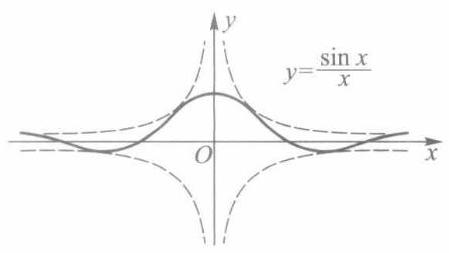
\includegraphics[width=.3\textwidth]{images/P011.jpg}
    \caption{图 $3-5$}
    \label{fig:P011}
\end{figure}

%例 1
\begin{example}
求 \(\mathop{\lim }\limits_{{x \rightarrow  \pi }}\frac{\sin x}{\pi  - x}\) .
\end{example}


%解
\begin{solution}
令 \(t = \pi  - x\) ,则 \(\sin x = \sin \left( {\pi  - t}\right)  = \sin t\) ,且当 \(x \rightarrow  \pi\) 时 \(t \rightarrow  0\) . 所以有
\[
\mathop{\lim }\limits_{{x \rightarrow  \pi }}\frac{\sin x}{\pi  - x} = \mathop{\lim }\limits_{{t \rightarrow  0}}\frac{\sin t}{t} = 1.
\]
\end{solution}

%例 2
\begin{example}
求 \(\mathop{\lim }\limits_{{x \rightarrow  0}}\frac{1 - \cos x}{{x}^{2}}\) .
\end{example}


%解
\begin{solution}
\[
\mathop{\lim }\limits_{{x \rightarrow  0}}\frac{1 - \cos x}{{x}^{2}} = \mathop{\lim }\limits_{{x \rightarrow  0}}\frac{1}{2}{\left( \frac{\sin \frac{x}{2}}{\frac{x}{2}}\right) }^{2} = \frac{1}{2}.
\]

\end{solution}


\subsection{证明 \(\mathop{\lim }\limits_{{x \rightarrow  \infty }}{\left( 1 + \frac{1}{x}\right) }^{x} = \mathrm{e}\)}
%证
\begin{proof}
所求证的极限等价于同时成立以下两个极限:
\[
\mathop{\lim }\limits_{{x \rightarrow   + \infty }}{\left( 1 + \frac{1}{x}\right) }^{x} = \mathrm{e}, \tag{2}
\]
\[
\mathop{\lim }\limits_{{x \rightarrow   - \infty }}{\left( 1 + \frac{1}{x}\right) }^{x} = \mathrm{e} \tag{3}
\]
先利用数列极限 \(\mathop{\lim }\limits_{{n \rightarrow  \infty }}{\left( 1 + \frac{1}{n}\right) }^{n} = \mathrm{e}\) 证明 (2) 式成立.

因为 \(\mathop{\lim }\limits_{{n \rightarrow  \infty }}{\left( 1 + \frac{1}{n + 1}\right) }^{n} = \mathop{\lim }\limits_{{n \rightarrow  \infty }}{\left( 1 + \frac{1}{n}\right) }^{n + 1} = \mathrm{e}\) ,所以对任意正数 \(\varepsilon\) ,存在正整数 \(N\) ,当 \(n \geq  N\) 时, 有
\[
\mathrm{e} - \varepsilon  < {\left( 1 + \frac{1}{n + 1}\right) }^{n} < {\left( 1 + \frac{1}{n}\right) }^{n + 1} < \mathrm{e} + \varepsilon . \tag{4}
\]
取 \(X = N\) ,当 \(x > X\) 时,令 \(n = \left\lbrack  x\right\rbrack\) ,那么
\[
{\left( 1 + \frac{1}{n + 1}\right) }^{n} < {\left( 1 + \frac{1}{x}\right) }^{x} < {\left( 1 + \frac{1}{n}\right) }^{n + 1}.
\]
由 (4) 式有
\[
\mathrm{e} - \varepsilon  < {\left( 1 + \frac{1}{x}\right) }^{x} < \mathrm{e} + \varepsilon ,
\]
这就证明了 \(\mathop{\lim }\limits_{{x \rightarrow   + \infty }}{\left( 1 + \frac{1}{x}\right) }^{x} = \mathrm{e}\) .

现证 (3) 式. 为此作代换 \(x =  - y\) ,则
\[
{\left( 1 + \frac{1}{x}\right) }^{x} = {\left( 1 - \frac{1}{y}\right) }^{-y} = {\left( 1 + \frac{1}{y - 1}\right) }^{y},
\]
且当 \(x \rightarrow   - \infty\) 时 \(y \rightarrow   + \infty\) ,从而有
\[
\mathop{\lim }\limits_{{x \rightarrow   - \infty }}{\left( 1 + \frac{1}{x}\right) }^{x} = \mathop{\lim }\limits_{{y \rightarrow   + \infty }}{\left( 1 + \frac{1}{y - 1}\right) }^{y - 1} \cdot  \left( {1 + \frac{1}{y - 1}}\right)  = \mathrm{e}.
\]
\end{proof}

以后还常用到 \(\mathrm{e}\) 的另一种极限形式:
\[
\mathop{\lim }\limits_{{\alpha  \rightarrow  0}}{\left( 1 + \alpha \right) }^{\frac{1}{\alpha }} = \mathrm{e} \tag{5}
\]
事实上,令 \(\alpha  = \frac{1}{x}\) ,则 \(x \rightarrow  \infty  \Leftrightarrow  \alpha  \rightarrow  0\) ,所以
\[
\mathrm{e} = \mathop{\lim }\limits_{{x \rightarrow  \infty }}{\left( 1 + \frac{1}{x}\right) }^{x} = \mathop{\lim }\limits_{{\alpha  \rightarrow  0}}{\left( 1 + \alpha \right) }^{\frac{1}{\alpha }}.
\]

%例 3
\begin{example}
求 \(\mathop{\lim }\limits_{{x \rightarrow  0}}{\left( 1 + 2x\right) }^{\frac{1}{x}}\) .
\end{example}


%解
\begin{solution}
\(\mathop{\lim }\limits_{{x \rightarrow  0}}{\left( 1 + 2x\right) }^{\frac{1}{x}} = \mathop{\lim }\limits_{{x \rightarrow  0}}\left\lbrack  {{\left( 1 + 2x\right) }^{\frac{1}{2x}} \cdot  {\left( 1 + 2x\right) }^{\frac{1}{2x}}}\right\rbrack   = {\mathrm{e}}^{2}\) .
\end{solution}


%例 4
\begin{example}
求 \(\mathop{\lim }\limits_{{x \rightarrow  0}}{\left( 1 - x\right) }^{\frac{1}{x}}\) .
\end{example}


%解
\begin{solution}
令 \(u =  - x\) ,则当 \(x \rightarrow  0\) 时 \(u \rightarrow  0\) . 因此
\[
\mathop{\lim }\limits_{{x \rightarrow  0}}{\left( 1 - x\right) }^{\frac{1}{x}} = \mathop{\lim }\limits_{{u \rightarrow  0}}{\left( 1 + u\right) }^{-\frac{1}{u}} = \frac{1}{\mathrm{e}}.
\]
\end{solution}

%例 5
\begin{example}
求 \(\mathop{\lim }\limits_{{n \rightarrow  \infty }}{\left( 1 + \frac{1}{n} - \frac{1}{{n}^{2}}\right) }^{n}\) .
\end{example}


%解
\begin{solution}
\({\left( 1 + \frac{1}{n} - \frac{1}{{n}^{2}}\right) }^{n} < {\left( 1 + \frac{1}{n}\right) }^{n} \rightarrow  \mathrm{e}\left( {n \rightarrow  \infty }\right)\) . 另一方面,当 \(n > 1\) 时有
\[
{\left( 1 + \frac{1}{n} - \frac{1}{{n}^{2}}\right) }^{n} = {\left( 1 + \frac{n - 1}{{n}^{2}}\right) }^{\frac{{n}^{2}}{n - 1} - \frac{n}{n - 1}} \geq  {\left( 1 + \frac{n - 1}{{n}^{2}}\right) }^{\frac{{n}^{2}}{n - 1} - 2},
\]
而由归结原则 \(\left( {\text{ 取 }{x}_{n} = \frac{{n}^{2}}{n - 1},n = 2,3,\cdots }\right)\) ,
\[
\mathop{\lim }\limits_{{n \rightarrow  \infty }}{\left( 1 + \frac{n - 1}{{n}^{2}}\right) }^{\frac{{n}^{2}}{n - 1} - 2} = \mathop{\lim }\limits_{{n \rightarrow  \infty }}{\left( 1 + \frac{n - 1}{{n}^{2}}\right) }^{\frac{{n}^{2}}{n - 1}}
\]
\[
= \mathop{\lim }\limits_{{x \rightarrow   + \infty }}{\left( 1 + \frac{1}{x}\right) }^{x} = \mathrm{e}.
\]
于是, 由数列极限的迫敛性得
\[
\mathop{\lim }\limits_{{n \rightarrow  \infty }}{\left( 1 + \frac{1}{n} - \frac{1}{{n}^{2}}\right) }^{n} = \mathrm{e}.
\]
\end{solution}

\subsection{习题 3.4}

1. 求下列极限:

(1) \(\mathop{\lim }\limits_{{x \rightarrow  0}}\frac{\sin {2x}}{x}\) ;

(2) \(\mathop{\lim }\limits_{{x \rightarrow  0}}\frac{\sin {x}^{3}}{{\left( \sin x\right) }^{2}}\) ;

(3) \(\mathop{\lim }\limits_{{x \rightarrow  \frac{\pi }{2}}}\frac{\cos x}{x - \frac{\pi }{2}}\) ;

(4) \(\mathop{\lim }\limits_{{x \rightarrow  0}}\frac{\tan x}{x}\) ;

(5) \(\mathop{\lim }\limits_{{x \rightarrow  0}}\frac{\tan x - \sin x}{{x}^{3}}\) ;

(6) \(\mathop{\lim }\limits_{{x \rightarrow  0}}\frac{\arctan x}{x}\) ;

(7) \(\mathop{\lim }\limits_{{x \rightarrow   + \infty }}x\sin \frac{1}{x}\) ;

(8) \(\mathop{\lim }\limits_{{x \rightarrow  a}}\frac{{\sin }^{2}x - {\sin }^{2}a}{x - a}\) ;

(9) \(\mathop{\lim }\limits_{{x \rightarrow  0}}\frac{\sin {4x}}{\sqrt{x + 1} - 1}\) ;

(10) \(\mathop{\lim }\limits_{{x \rightarrow  0}}\frac{\sqrt{1 - \cos {x}^{2}}}{1 - \cos x}\) .

2. 求下列极限:

(1) \(\mathop{\lim }\limits_{{x \rightarrow  \infty }}{\left( 1 - \frac{2}{x}\right) }^{-x}\) ;

(2) \(\mathop{\lim }\limits_{{x \rightarrow  0}}{\left( 1 + \alpha x\right) }^{\frac{1}{x}}\) (α为给定实数);

(3) \(\mathop{\lim }\limits_{{x \rightarrow  0}}{\left( 1 + \tan x\right) }^{\cot x}\) ;

(4) \(\mathop{\lim }\limits_{{x \rightarrow  0}}{\left( \frac{1 + x}{1 - x}\right) }^{\frac{1}{x}}\) ;

(5) \(\mathop{\lim }\limits_{{x \rightarrow   + \infty }}{\left( \frac{{3x} + 2}{{3x} - 1}\right) }^{{2x} - 1}\) ;

(6) \(\mathop{\lim }\limits_{{x \rightarrow   + \infty }}{\left( 1 + \frac{\alpha }{x}\right) }^{\beta x}\left( {\alpha ,\beta \text{ 为给定实数 }}\right)\) .

3. 证明: \(\mathop{\lim }\limits_{{x \rightarrow  0}}\left\{  {\mathop{\lim }\limits_{{n \rightarrow  \infty }}\left\lbrack  {\cos x\cos \frac{x}{2}\cos \frac{x}{{2}^{2}}\cdots \cos \frac{x}{{2}^{n}}}\right\rbrack  }\right\}   = 1\) .

4. 利用归结原则计算下列极限:

(1) \(\mathop{\lim }\limits_{{n \rightarrow  \infty }}\sqrt{n}\sin \frac{\pi }{n}\) ;

(2) \(\mathop{\lim }\limits_{{n \rightarrow  \infty }}{\left( 1 + \frac{1}{n} + \frac{1}{{n}^{2}}\right) }^{n}\) .

\section{无穷小量与无穷大量}

\subsection{无穷小量}

与无穷小数列的概念相类似, 我们给出关于函数为无穷小量的定义.

%定义  1
\begin{definition}{函数的无穷小量}{def:函数的无穷小量}
设 \(f\) 在某 \({U}^{ \circ  }\left( {x}_{0}\right)\) 上有定义. 若
\[
\mathop{\lim }\limits_{{x \rightarrow  {x}_{0}}}f\left( x\right)  = 0,
\]
则称 \(f\) 为当 \(x \rightarrow  {x}_{0}\) 时的无穷小量.
\end{definition}


若函数 \(g\) 在某 \({U}^{ \circ  }\left( {x}_{0}\right)\) 上有界,则称 \(g\) 为当 \(x \rightarrow  {x}_{0}\) 时的有界量.

类似地,定义当 \(x \rightarrow  {x}_{0}^{ + },x \rightarrow  {x}_{0}^{ - },x \rightarrow   + \infty ,x \rightarrow   - \infty\) 以及 \(x \rightarrow  \infty\) 时的无穷小量与有界量.

例如, \({x}^{2},\sin x\) 与 \(1 - \cos x\) 都是当 \(x \rightarrow  0\) 时的无穷小量, \(\sqrt{1 - x}\) 是当 \(x \rightarrow  1\) 时的无穷小量,而 \(\frac{1}{{x}^{2}},\frac{\sin x}{x}\) 为 \(x \rightarrow  \infty\) 时的无穷小量. 又如 \(\sin x\) 是当 \(x \rightarrow  \infty\) 时的有界量, \(\sin \frac{1}{x}\) 是当 \(x \rightarrow\) 0 时的有界量. 特别地, 任何无穷小量也必都是有界量.

由无穷小量的定义可立刻推得如下性质:

1. 两个 (相同类型的) 无穷小量之和、差、积仍为无穷小量.

2. 无穷小量与有界量的乘积为无穷小量.

例如,当 \(x \rightarrow  0\) 时, \({x}^{2}\) 是无穷小量, \(\sin \frac{1}{x}\) 为有界量,故由性质 2 即得
\[
\mathop{\lim }\limits_{{x \rightarrow  0}}{x}^{2}\sin \frac{1}{x} = 0.
\]

\begin{figure}
	\centering
	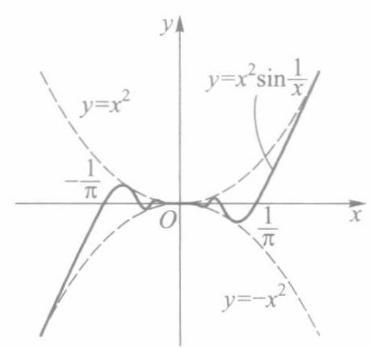
\includegraphics[width=.3\textwidth]{images/P012.jpg}
	\caption{图 $3-6$}
	\label{fig:P012}
\end{figure}

函数 \(y = {x}^{2}\sin \frac{1}{x}\) 的图像如图 3-6 所示.

由函数极限与无穷小量的定义可立即推出如下结论:

\(\mathop{\lim }\limits_{{x \rightarrow  {x}_{0}}}f\left( x\right)  = A \Leftrightarrow  f\left( x\right)  - A\) 是当 \(x \rightarrow  {x}_{0}\) 时的无穷小量.

\subsection{无穷小量阶的比较}

无穷小量是以 0 为极限的函数, 而不同的无穷小量收敛于 0 的速度有快有慢. 为此, 我们考察两个无穷小量的比, 以便对它们的收敛速度作出判断.

设当 \(x \rightarrow  {x}_{0}\) 时, \(f\) 与 \(g\) 均为无穷小量.

1. 若 \(\mathop{\lim }\limits_{{x \rightarrow  {x}_{0}}}\frac{f\left( x\right) }{g\left( x\right) } = 0\) ,则称当 \(x \rightarrow  {x}_{0}\) 时 \(f\) 为 \(g\) 的高阶无穷小量,或称 \(g\) 为 \(f\) 的低阶无穷小量, 记作
\[
f\left( x\right)  = o\left( {g\left( x\right) }\right) \left( {x \rightarrow  {x}_{0}}\right) .
\]
特别地, \(f\) 为当 \(x \rightarrow  {x}_{0}\) 时的无穷小量记作
\[
f\left( x\right)  = o\left( 1\right) \left( {x \rightarrow  {x}_{0}}\right) .
\]

例如,当 \(x \rightarrow  0\) 时, \(x,{x}^{2},\cdots ,{x}^{n}\) ( \(n\) 为正整数) 等都是无穷小量,因而有
\[
{x}^{k} = o\left( 1\right) \left( {x \rightarrow  0}\right) ,k = 1,2,\cdots ,
\]
而且它们中后一个为前一个的高阶无穷小量, 即有
\[
{x}^{k + 1} = o\left( {x}^{k}\right) \left( {x \rightarrow  0}\right) .
\]
又如,由于 \(\mathop{\lim }\limits_{{x \rightarrow  0}}\frac{1 - \cos x}{\sin x} = \mathop{\lim }\limits_{{x \rightarrow  0}}\tan \frac{x}{2} = 0\) . 故有
\[
1 - \cos x = o\left( {\sin x}\right) \left( {x \rightarrow  0}\right) .
\]

2. 若存在正数 \(K\) 和 \(L\) ,使得在某 \({U}^{ \circ  }\left( {x}_{0}\right)\) 上有
\[
K \leq  \left| \frac{f\left( x\right) }{g\left( x\right) }\right|  \leq  L,
\]
则称 \(f\) 与 \(g\) 为当 \(x \rightarrow  {x}_{0}\) 时的同阶无穷小量. 特别当
\[
\mathop{\lim }\limits_{{x \rightarrow  {x}_{0}}}\frac{f\left( x\right) }{g\left( x\right) } = c \neq  0
\]
时, \(f\) 与 \(g\) 必为同阶无穷小量.

例如,当 \(x \rightarrow  0\) 时, \(1 - \cos x\) 与 \({x}^{2}\) 皆为无穷小量. 由于
\[
\mathop{\lim }\limits_{{x \rightarrow  0}}\frac{1 - \cos x}{{x}^{2}} = \frac{1}{2},
\]
所以 \(1 - \cos x\) 与 \({x}^{2}\) 为当 \(x \rightarrow  0\) 时的同阶无穷小量. 又如,当 \(x \rightarrow  0\) 时, \(x\) 与 \(x\left( {2 + \sin \frac{1}{x}}\right)\) 都是无穷小量, 由于它们之比的绝对值满足
\[
1 \leq  \left| {2 + \sin \frac{1}{x}}\right|  \leq  3,
\]
所以 \(x\) 与 \(x\left( {2 + \sin \frac{1}{x}}\right)\) 为当 \(x \rightarrow  0\) 时的同阶无穷小量.

若无穷小量 \(f\) 与 \(g\) 满足关系式
\[
\left| \frac{f\left( x\right) }{g\left( x\right) }\right|  \leq  L,\;x \in  {U}^{ \circ  }\left( {x}_{0}\right) ,
\]
则记作
\[
f\left( x\right)  = O\left( {g\left( x\right) }\right) \left( {x \rightarrow  {x}_{0}}\right) .
\]
特别地,若 \(f\) 在某 \({U}^{ \circ  }\left( {x}_{0}\right)\) 上有界,则记为
\[
f\left( x\right)  = O\left( 1\right) \left( {x \rightarrow  {x}_{0}}\right) .
\]
例如,
\[
1 - \cos x = O\left( {x}^{2}\right) \left( {x \rightarrow  0}\right) ,
\]
\[
x\left( {2 + \sin \frac{1}{x}}\right)  = O\left( x\right) \left( {x \rightarrow  0}\right) ,
\]
\[
\sin x = O\left( 1\right) \left( {x \rightarrow  \infty }\right) \text{ . }
\]
甚至当 \(f\left( x\right)  = o\left( {g\left( x\right) }\right) \left( {x \rightarrow  {x}_{0}}\right)\) 时,也有 \(f\left( x\right)  = O\left( {g\left( x\right) }\right) \left( {x \rightarrow  {x}_{0}}\right)\) .

%注
\begin{remark}
本段中的等式 \(f\left( x\right)  = o\left( {g\left( x\right) }\right) \left( {x \rightarrow  {x}_{0}}\right)\) 与 \(f\left( x\right)  = O\left( {g\left( x\right) }\right) \left( {x \rightarrow  {x}_{0}}\right)\) 等,与通常等式的含义是不同的. 这里等式左边是一个函数, 右边是一个函数类, 而中间的等号的含义是“属于”. 例如, 前面已经得到
\[
1 - \cos x = o\left( {\sin x}\right) \left( {x \rightarrow  0}\right) , \tag{1}
\]
其中
\[
o\left( {\sin x}\right)  = \left\{  {f\left| {\;\mathop{\lim }\limits_{{x \rightarrow  0}}\frac{f\left( x\right) }{\sin x} = 0}\right. }\right\}  ,
\]
等式 (1) 表示函数 \(1 - \cos x\) 属于此函数类.
\end{remark}


3. 若 \(\mathop{\lim }\limits_{{x \rightarrow  {x}_{0}}}\frac{f\left( x\right) }{g\left( x\right) } = 1\) ,则称 \(f\) 与 \(g\) 是当 \(x \rightarrow  {x}_{0}\) 时的等价无穷小量. 记作
\[
f\left( x\right)  \sim  g\left( x\right) \left( {x \rightarrow  {x}_{0}}\right) .
\]
例如,由于 \(\mathop{\lim }\limits_{{x \rightarrow  0}}\frac{\sin x}{x} = 1\) ,故有 \(\sin x \sim  x\left( {x \rightarrow  0}\right)\) . 又由于 \(\mathop{\lim }\limits_{{x \rightarrow  0}}\frac{\arctan x}{x} = 1\) (上节习题 1 (6)),故有 \(\arctan x \sim  x\left( {x \rightarrow  0}\right)\) .

以上讨论了两个无穷小量阶的比较. 但应指出, 并不是任何两个无穷小量都可以进行这种阶的比较. 例如,当 \(x \rightarrow  0\) 时, \(x\sin \frac{1}{x}\) 和 \({x}^{2}\) 都是无穷小量,但它们的比
\[
\frac{x\sin \frac{1}{x}}{{x}^{2}} = \frac{1}{x}\sin \frac{1}{x}\text{ 或 }\frac{{x}^{2}}{x\sin \frac{1}{x}} = \frac{x}{\sin \frac{1}{x}}
\]
当 \(x \rightarrow  0\) 时都不是有界量,所以这两个无穷小量不能进行阶的比较.

下述定理显示了等价无穷小量在求极限问题中的作用.

%定理 3.12
\begin{theorem}{等价无穷小量的作用}{the:等价无穷小量的作用}
设函数 \(f,g,h\) 在 \({U}^{ \circ  }\left( {x}_{0}\right)\) 上有定义,且有
\[
f\left( x\right)  \sim  g\left( x\right) \left( {x \rightarrow  {x}_{0}}\right) .
\]
(i) 若 \(\mathop{\lim }\limits_{{x \rightarrow  {x}_{0}}}f\left( x\right) h\left( x\right)  = A\) ,则 \(\mathop{\lim }\limits_{{x \rightarrow  {x}_{0}}}g\left( x\right) h\left( x\right)  = A\) ;

(ii) 若 \(\mathop{\lim }\limits_{{x \rightarrow  {x}_{0}}}\frac{h\left( x\right) }{f\left( x\right) } = B\) ,则 \(\mathop{\lim }\limits_{{x \rightarrow  {x}_{0}}}\frac{h\left( x\right) }{g\left( x\right) } = B\) .
\end{theorem}

%证
\begin{proof}
(i) \(\mathop{\lim }\limits_{{x \rightarrow  {x}_{0}}}g\left( x\right) h\left( x\right)  = \mathop{\lim }\limits_{{x \rightarrow  {x}_{0}}}\frac{g\left( x\right) }{f\left( x\right) } \cdot  \mathop{\lim }\limits_{{x \rightarrow  {x}_{0}}}f\left( x\right) h\left( x\right)  = 1 \cdot  A = A\) .

(ii) 可类似地证明.
\end{proof}


%例 1
\begin{example}
求 \(\mathop{\lim }\limits_{{x \rightarrow  0}}\frac{\arctan x}{\sin {4x}}\) .
\end{example}


%解
\begin{solution}
由于 \(\arctan x \sim  x\left( {x \rightarrow  0}\right) ,\sin {4x} \sim  {4x}\left( {x \rightarrow  0}\right)\) . 故由定理 3.12 得
\[
\mathop{\lim }\limits_{{x \rightarrow  0}}\frac{\arctan x}{\sin {4x}} = \mathop{\lim }\limits_{{x \rightarrow  0}}\frac{x}{4x} = \frac{1}{4}.
\]
\end{solution}

%例 2
\begin{example}

\end{example}
利用等价无穷小量代换求极限
\[
\mathop{\lim }\limits_{{x \rightarrow  0}}\frac{\tan x - \sin x}{\sin {x}^{3}}.
\]
%解
\begin{solution}
由于 \(\tan x - \sin x = \frac{\sin x}{\cos x}\left( {1 - \cos x}\right)\) ,而
\[
\sin x \sim  x\left( {x \rightarrow  0}\right) ,1 - \cos x \sim  \frac{{x}^{2}}{2}\left( {x \rightarrow  0}\right) ,\sin {x}^{3} \sim  {x}^{3}\left( {x \rightarrow  0}\right) ,
\]
故有
\[
\mathop{\lim }\limits_{{x \rightarrow  0}}\frac{\tan x - \sin x}{\sin {x}^{3}} = \mathop{\lim }\limits_{{x \rightarrow  0}}\frac{1}{\cos x} \cdot  \frac{x \cdot  \frac{{x}^{2}}{2}}{{x}^{3}} = \frac{1}{2}.
\]
\end{solution}

%注
\begin{remark}
在利用等价无穷小量代换求极限时, 应注意: 只有对所求极限式中相乘或相除的因式才能用等价无穷小量来替代, 而对极限式中的相加或相减部分则不能随意替代. 如在例 2 中, 若因有
\[
\tan x \sim  x\left( {x \rightarrow  0}\right) ,\sin x \sim  x\left( {x \rightarrow  0}\right) ,
\]
而推出
\[
\mathop{\lim }\limits_{{x \rightarrow  0}}\frac{\tan x - \sin x}{\sin {x}^{3}} = \mathop{\lim }\limits_{{x \rightarrow  0}}\frac{x - x}{\sin {x}^{3}} = 0,
\]
则得到的是错误的结果.
\end{remark}


\subsection{无穷大量}

%定义  2
\begin{definition}{非正常极限}{def:非正常极限}
设函数 \(f\) 在某 \({U}^{ \circ  }\left( {x}_{0}\right)\) 上有定义. 若对任给的 \(G > 0\) ,存在 \(\delta  > 0\) ,使得当 \(x \in\)  \({U}^{ \circ  }\left( {{x}_{0};\delta }\right) \left( { \subset  {U}^{ \circ  }\left( {x}_{0}\right) }\right)\) 时,有
\[
\left| {f\left( x\right) }\right|  > G, \tag{2}
\]
则称函数 \(f\) 当 \(x \rightarrow  {x}_{0}\) 时有非正常极限 \(\infty\) ,记作
\[
\mathop{\lim }\limits_{{x \rightarrow  {x}_{0}}}f\left( x\right)  = \infty .
\]
若 (2) 式换成 “ \(f\left( x\right)  > G\) ” 或 “ \(f\left( x\right)  <  - G\) ”,则分别称 \(f\) 当 \(x \rightarrow  {x}_{0}\) 时有非正常极限 \(+ \infty\) 或 \(- \infty\) , 记作
\[
\mathop{\lim }\limits_{{x \rightarrow  {x}_{0}}}f\left( x\right)  =  + \infty \text{ 或 }\mathop{\lim }\limits_{{x \rightarrow  {x}_{0}}}f\left( x\right)  =  - \infty .
\]
\end{definition}

关于函数 \(f\) 在自变量 \(x\) 的其他不同趋向的非正常极限的定义,以及数列 \(\left\{  {a}_{n}\right\}\) 当 \(n \rightarrow  \infty\) 时的非正常极限的定义,都可类似地给出. 例如:

\(\mathop{\lim }\limits_{{x \rightarrow   + \infty }}f\left( x\right)  =  - \infty\) 的定义: 任给 \(G > 0\) ,存在 \(M > 0\) ,使得当 \(x > M\) 时,有 \(f\left( x\right)  <  - G\) ;

\(\mathop{\lim }\limits_{{n \rightarrow  \infty }}{a}_{n} =  + \infty\) 的定义: 任给 \(G > 0\) ,存在 \(N > 0\) ,使得当 \(n > N\) 时,有 \({a}_{n} > G\) .

%定义  3
\begin{definition}{无穷大量}{def:无穷大量}
对于自变量 \(x\) 的某种趋向 (或 \(n \rightarrow  \infty\) 时),所有以 \(\infty , + \infty\) 或 \(- \infty\) 为非正常极限的函数 (包括数列), 都称为无穷大量.
\end{definition}


%例 3
\begin{example}
证明 \(\mathop{\lim }\limits_{{x \rightarrow  0}}\frac{1}{{x}^{2}} =  + \infty\) .
\end{example}


%证
\begin{proof}
任给 \(G > 0\) ,要使 \(\frac{1}{{x}^{2}} > G\) ,只要 \(\left| x\right|  < \frac{1}{\sqrt{G}}\) ,因此令 \(\delta  = \frac{1}{\sqrt{G}}\) ,则对一切 \(x \in  {U}^{ \circ  }\left( {0;\delta }\right)\) ,有 \(\frac{1}{{x}^{2}} > G\) . 这就证明了 \(\mathop{\lim }\limits_{{x \rightarrow  0}}\frac{1}{{x}^{2}} =  + \infty\) .
\end{proof}


%例 4
\begin{example}
证明: 当 \(a > 1\) 时, \(\mathop{\lim }\limits_{{x \rightarrow   + \infty }}{a}^{x} =  + \infty\) .
\end{example}


%证
\begin{proof}
任给 \(G > 0\) (不妨设 \(G > 1\) ),要使 \({a}^{x} > G\) ,由对数函数的严格增性,只要 \(x > {\log }_{a}G\) , 因此令 \(M = {\log }_{a}G\) ,则对一切 \(x > M\) ,有 \({a}^{x} > G\) . 这就证得 \(\mathop{\lim }\limits_{{x \rightarrow   + \infty }}{a}^{x} =  + \infty\) .
\end{proof}


顺便指出,容易证明: 当 \(a > 1\) 时, \(\mathop{\lim }\limits_{{x \rightarrow   - \infty }}{a}^{x} = 0\) ; 当 \(0 < a < 1\) 时,有
\[
\mathop{\lim }\limits_{{x \rightarrow   + \infty }}{a}^{x} = 0,\;\mathop{\lim }\limits_{{x \rightarrow   - \infty }}{a}^{x} =  + \infty .
\]
%注
\begin{remark}
1 无穷大量不是很大的数,而是具有非正常极限的函数. 如由例 3 知 \(\frac{1}{{x}^{2}}\) 是当 \(x \rightarrow  0\) 时的无穷大量,由例 4 知 \({a}^{x}\left( {a > 1}\right)\) 是当 \(x \rightarrow   + \infty\) 时的无穷大量.
\end{remark}


%注
\begin{remark}
2 若 \(f\) 为 \(x \rightarrow  {x}_{0}\) 时的无穷大量,则易见 \(f\) 为 \({U}^{ \circ  }\left( {x}_{0}\right)\) 上的无界函数. 但无界函数却不一定是无穷大量. 如 \(f\left( x\right)  = x\sin x\) 在 \(U\left( {+\infty }\right)\) 上无界,因对任给的 \(G > 0\) ,取 \({x}_{n} = {2n\pi } +\)  \(\frac{\pi }{2}\) ,这里正整数 \(n > \frac{G}{2\pi }\) ,则有
\[
f\left( {x}_{n}\right)  = \left( {{2n\pi } + \frac{\pi }{2}}\right) \sin \left( {{2n\pi } + \frac{\pi }{2}}\right)  = {2n\pi } + \frac{\pi }{2} > \mathrm{G}.
\]
但 \(\mathop{\lim }\limits_{{x \rightarrow   + \infty }}f\left( x\right)  \neq  \infty\) ,因若取数列 \({x}_{n}^{ * } = {2n\pi }\left( {n = 1,2,\cdots }\right)\) ,则 \({x}_{n}^{ * } \rightarrow   + \infty \left( {n \rightarrow  \infty }\right)\) ,而
\[
\mathop{\lim }\limits_{{n \rightarrow   + \infty }}f\left( {x}_{n}^{ * }\right)  = 0.
\]
\end{remark}

%例 5
\begin{example}
设 \(f\left( x\right)\) 为 \(x \rightarrow  {x}_{0}\) 时的无穷大量, \(g\left( x\right)\) 在 \(U\left( {x}_{0}\right)\) 上满足 \(\left| {g\left( x\right) }\right|  \geq  K > 0\) . 证明: \(f\left( x\right) g\left( x\right)\) 为 \(x \rightarrow  {x}_{0}\) 时的无穷大量。
\end{example}


%证
\begin{proof}
因为 \(\mathop{\lim }\limits_{{x \rightarrow  {x}_{0}}}f\left( x\right)  = \infty\) ,则对任给 \(G > 0\) ,存在 \(\delta  > 0\) ,当 \(0 < \left| {x - {x}_{0}}\right|  < \delta\) 时,有
\[
\left| {f\left( x\right) }\right|  > \frac{G}{K}.
\]
那么
\[
\left| {f\left( x\right) g\left( x\right) }\right|  > \frac{G}{K} \cdot  K = G,
\]
这就说明 \(\mathop{\lim }\limits_{{x \rightarrow  {x}_{0}}}f\left( x\right) g\left( x\right)  = \infty\) .
\end{proof}


如同对无穷小量进行阶的比较的讨论一样, 对两个无穷大量也可定义高阶无穷大量、同阶无穷大量等概念. 这里就不再详述了.

由无穷大量与无穷小量的定义, 可推得它们之间有如下关系:

%定理 3.13
\begin{theorem}{无穷大量与无穷小量的关系}{the:无穷大量与无穷小量的关系}
(i) 设 \(f\) 在 \({U}^{ \circ  }\left( {x}_{0}\right)\) 上有定义且不等于 0 . 若 \(f\) 为 \(x \rightarrow  {x}_{0}\) 时的无穷小量, 则 \(\frac{1}{f}\) 为 \(x \rightarrow  {x}_{0}\) 时的无穷大量.

(ii) 若 \(g\) 为 \(x \rightarrow  {x}_{0}\) 时的无穷大量,则 \(\frac{1}{g}\) 为 \(x \rightarrow  {x}_{0}\) 时的无穷小量.
\end{theorem}

定理的证明留给读者. 根据这个定理, 对无穷大量的研究可归结为对无穷小量的讨论.

\subsection{曲线的渐近线}

作为函数极限的一个应用, 我们讨论曲线的渐近线问题. 由平面解析几何知道, 双曲线 \(\frac{{x}^{2}}{{a}^{2}} - \frac{{y}^{2}}{{b}^{2}} = 1\) 有两条渐近线 \(\frac{x}{a} \pm  \frac{y}{b} = 0\) (图 3-7). 一般地,曲线的渐近线定义如下.

%定义  4
\begin{definition}{渐近线}{def:渐近线}
若曲线 \(C\) 上的动点 \(P\) 沿着曲线无限地远离原点时,点 \(P\) 与某定直线 \(L\) 的距离趋于 0,则称直线 \(L\) 为曲线 \(C\) 的渐近线 (图 3-8).
\end{definition}


\begin{figure}
	\centering
	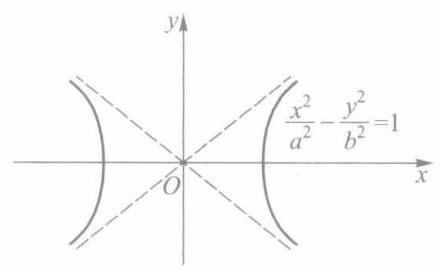
\includegraphics[width=.3\textwidth]{images/P013.jpg}
	\caption{图 $3-7$}
	\label{fig:P013}
\end{figure}

\begin{figure}
	\centering
	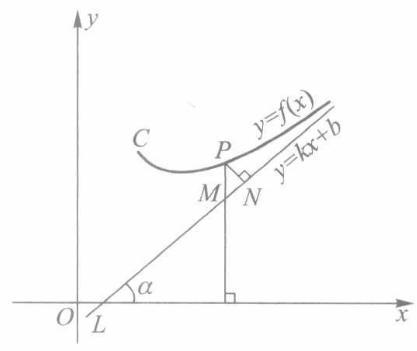
\includegraphics[width=.3\textwidth]{images/P014.jpg}
	\caption{图 $3-8$}
	\label{fig:P014}
\end{figure}

下面我们讨论曲线 \(y = f\left( x\right)\) 在什么条件下存在斜渐近线 \(y = {kx} + b\) 与垂直渐近线 \(x =\)  \({x}_{0}\) ,以及怎样求出渐近线方程.

现假设曲线 \(y = f\left( x\right)\) 有斜渐近线 \(y = {kx} + b\) . 如图 3-8 所示,曲线上动点 \(P\) 到渐近线的距离为
\[
\left| {PN}\right|  = \left| {{PM}\cos \alpha }\right|  = \left| {f\left( x\right)  - \left( {{kx} + b}\right) }\right| \frac{1}{\sqrt{1 + {k}^{2}}}.
\]
按渐近线的定义,当 \(x \rightarrow   + \infty\) 时 \footnote{对于 \(x \rightarrow   - \infty\) 或 \(x \rightarrow  \infty\) 的情形,也有相应的结果.} \(\left| {PN}\right|  \rightarrow  0\) ,即有
\[
\mathop{\lim }\limits_{{x \rightarrow   + \infty }}\left\lbrack  {f\left( x\right)  - \left( {{kx} + b}\right) }\right\rbrack   = 0,
\]
或
\[
\mathop{\lim }\limits_{{x \rightarrow   + \infty }}\left\lbrack  {f\left( x\right)  - {kx}}\right\rbrack   = b. \tag{3}
\]
又由
\[
\mathop{\lim }\limits_{{x \rightarrow   + \infty }}\left\lbrack  {\frac{f\left( x\right) }{x} - k}\right\rbrack   = \mathop{\lim }\limits_{{x \rightarrow   + \infty }}\frac{1}{x}\left\lbrack  {f\left( x\right)  - {kx}}\right\rbrack   = 0 \cdot  b = 0,
\]


得到
\[
\mathop{\lim }\limits_{{x \rightarrow   + \infty }}\frac{f\left( x\right) }{x} = k. \tag{4}
\]
由上面的讨论可知,若曲线 \(y = f\left( x\right)\) 有斜渐近线 \(y = {kx} + b\) ,则常数 \(k\) 与 \(b\) 可相继由 (4) 式和 (3) 式来确定; 反之,若由 (4)、(3) 两式求得 \(k\) 与 \(b\) ,则可知 \(\left| {PN}\right|  \rightarrow  0(x \rightarrow\)  \(+ \infty )\) ,从而 \(y = {kx} + b\) 为曲线 \(y = f\left( x\right)\) 的渐近线.

若函数 \(f\) 满足
\[
\mathop{\lim }\limits_{{x \rightarrow  {x}_{0}}}f\left( x\right)  = \infty \;\left( {\text{ 或 }\mathop{\lim }\limits_{{x \rightarrow  {x}_{0}^{ + }}}f\left( x\right)  = \infty ,\mathop{\lim }\limits_{{x \rightarrow  {x}_{0}^{ - }}}f\left( x\right)  = \infty }\right) ,
\]
则按渐近线的定义可知,曲线 \(y = f\left( x\right)\) 有垂直于 \(x\) 轴的渐近线 \(x = {x}_{0}\) ,称为垂直渐近线.

%例 6
\begin{example}
求曲线 \(f\left( x\right)  = \frac{{x}^{3}}{{x}^{2} + {2x} - 3}\) 的渐近线.
\end{example}


%解
\begin{solution}
由 (4) 式
\[
\frac{f\left( x\right) }{x} = \frac{{x}^{3}}{{x}^{3} + 2{x}^{2} - {3x}} \rightarrow  1\;\left( {x \rightarrow  \infty }\right) ,
\]
得 \(k = 1\) . 再由 (3) 式
\[
f\left( x\right)  - {kx} = \frac{{x}^{3}}{{x}^{2} + {2x} - 3} - x \rightarrow   - 2\;\left( {x \rightarrow  \infty }\right) ,
\]
得 \(b =  - 2\) . 从而求得此曲线的斜渐近线方程为 \(y = x - 2\) .

又由 \(f\left( x\right)  = \frac{{x}^{3}}{\left( {x + 3}\right) \left( {x - 1}\right) }\) 易见
\[
\mathop{\lim }\limits_{{x \rightarrow   - 3}}f\left( x\right)  = \infty ,\mathop{\lim }\limits_{{x \rightarrow  1}}f\left( x\right)  = \infty ,
\]
所以此曲线有垂直渐近线 \(x =  - 3\) 和 \(x = 1\) (图 3-9).

\begin{figure}
    \centering
    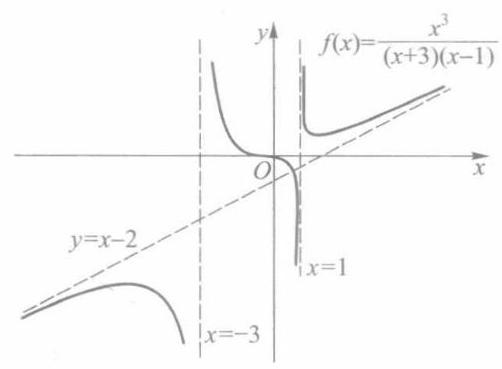
\includegraphics[width=.3\textwidth]{images/P015.jpg}
    \caption{图 $3-9$}
    \label{fig:P015}
\end{figure}
\end{solution}


\subsection{习题 3.5}

1. 证明下列各式:

(1) \({2x} - {x}^{2} = O\left( x\right) \left( {x \rightarrow  0}\right)\) ;

(2) \(x\sin \sqrt{x} = O\left( {x}^{\frac{3}{2}}\right) \;\left( {x \rightarrow  {0}^{ + }}\right)\) ;

(3) \(\sqrt{1 + x} - 1 = o\left( 1\right) \left( {x \rightarrow  0}\right)\) ;

(4) \({\left( 1 + x\right) }^{n} = 1 + {nx} + o\left( x\right) \left( {x \rightarrow  0}\right) \left( {n\text{ 为正整数 }}\right)\) ;

(5) \(2{x}^{3} + {x}^{2} = O\left( {x}^{3}\right) \left( {x \rightarrow  \infty }\right)\) ;

(6) \(o\left( {g\left( x\right) }\right)  \pm  o\left( {g\left( x\right) }\right)  = o\left( {g\left( x\right) }\right) \left( {x \rightarrow  {x}_{0}}\right)\) \footnote{这里等式的含义是:两个比 \(g\) 高阶的无穷小量的和或差仍是一个比 \(g\) 高阶的无穷小量.后一小题类似.}
;

(7) \(o\left( {{g}_{1}\left( x\right) }\right)  \cdot  o\left( {{g}_{2}\left( x\right) }\right)  = o\left( {{g}_{1}\left( x\right) {g}_{2}\left( x\right) }\right) \left( {x \rightarrow  {x}_{0}}\right)\) .

2. 应用定理 3.12 求下列极限:

(1) \(\mathop{\lim }\limits_{{x \rightarrow  \infty }}\frac{x\arctan \frac{1}{x}}{x - \cos x}\) ;

(2) \(\mathop{\lim }\limits_{{x \rightarrow  0}}\frac{\sqrt{1 + {x}^{2}} - 1}{1 - \cos x}\) .

3. 证明定理 3.13 .

4. 求下列函数所表示曲线的渐近线:

(1) \(y = \frac{1}{x}\) ;

(2) \(y = \arctan x\) ;

(3) \(y = \frac{3{x}^{3} + 4}{{x}^{2} - {2x}}\) .

5. 试确定 \(\alpha\) 的值,使下列函数与 \({x}^{\alpha }\) 当 \(x \rightarrow  0\) 时为同阶无穷小量:

(1) \(\sin {2x} - 2\sin x\) ;

(2) \(\frac{1}{1 + x} - \left( {1 - x}\right)\) ;

(3) \(\sqrt{1 + \tan x} - \sqrt{1 - \sin x}\) ; (4) \(\sqrt[5]{3{x}^{2} - 4{x}^{3}}\) .

6. 试确定 \(\alpha\) 的值,使下列函数与 \({x}^{\alpha }\) 当 \(x \rightarrow  \infty\) 时为同阶无穷大量:

(1) \(\sqrt{{x}^{2} + {x}^{5}}\) ；

(2) \(x + {x}^{2}\left( {2 + \sin x}\right)\) ;

(3) \(\left( {1 + x}\right) \left( {1 + {x}^{2}}\right) \cdots \left( {1 + {x}^{n}}\right)\) .

7. 证明: 若 \(S\) 为无上界数集,则存在一递增数列 \(\left\{  {x}_{n}\right\}   \subset  S\) ,使得 \({x}_{n} \rightarrow   + \infty \left( {n \rightarrow  \infty }\right)\) .

8. 设 \(\mathop{\lim }\limits_{{x \rightarrow  {x}_{0}}}f\left( x\right)  = \infty ,\mathop{\lim }\limits_{{x \rightarrow  {x}_{0}}}g\left( x\right)  = b \neq  0\) . 证明: \(\mathop{\lim }\limits_{{x \rightarrow  {x}_{0}}}f\left( x\right) g\left( x\right)  = \infty\) .

9. 设 \(f\left( x\right)  \sim  g\left( x\right) \left( {x \rightarrow  {x}_{0}}\right)\) ,证明:

\(f\left( x\right)  - g\left( x\right)  = o\left( {f\left( x\right) }\right)\) 或 \(f\left( x\right)  - g\left( x\right)  = o\left( {g\left( x\right) }\right) .\)

10. 写出并证明 \(\mathop{\lim }\limits_{{x \rightarrow   + \infty }}f\left( x\right)  =  + \infty\) 的归结原则.

\section{第三章总练习题}

1. 求下列极限:

(1) \(\mathop{\lim }\limits_{{x \rightarrow  {3}^{ - }}}\left( {x - \left\lbrack  x\right\rbrack  }\right)\) ;

(2) \(\mathop{\lim }\limits_{{x \rightarrow  {1}^{ + }}}{\left( \left\lbrack  x\right\rbrack   + 1\right) }^{-1}\) ;

(3) \(\mathop{\lim }\limits_{{x \rightarrow   + \infty }}\left( {\sqrt{\left( {a + x}\right) \left( {b + x}\right) } - \sqrt{\left( {a - x}\right) \left( {b - x}\right) }}\right)\) ;

(4) \(\mathop{\lim }\limits_{{x \rightarrow   + \infty }}\frac{x}{\sqrt{{x}^{2} - {a}^{2}}}\) ;

(5) \(\mathop{\lim }\limits_{{x \rightarrow   - \infty }}\frac{x}{\sqrt{{x}^{2} - {a}^{2}}}\) ;

(6) \(\mathop{\lim }\limits_{{x \rightarrow  0}}\frac{\sqrt{1 + x} - \sqrt{1 - x}}{\sqrt[3]{1 + x} - \sqrt[3]{1 - x}}\) ;

(7) \(\mathop{\lim }\limits_{{x \rightarrow  1}}\left( {\frac{m}{1 - {x}^{m}} - \frac{n}{1 - {x}^{n}}}\right) ,m,n\) 为正整数.

2. 分别求出满足下述条件的常数 \(a\) 与 \(b\) :

(1) \(\mathop{\lim }\limits_{{x \rightarrow   + \infty }}\left( {\frac{{x}^{2} + 1}{x + 1} - {ax} - b}\right)  = 0\) ;

(2) \(\mathop{\lim }\limits_{{x \rightarrow   - \infty }}\left( {\sqrt{{x}^{2} - x + 1} - {ax} - b}\right)  = 0\) ;

(3) \(\mathop{\lim }\limits_{{x \rightarrow   + \infty }}\left( {\sqrt{{x}^{2} - x + 1} - {ax} - b}\right)  = 0\) .

3. 试分别举出符合下列要求的函数 \(f\) :

(1) \(\mathop{\lim }\limits_{{x \rightarrow  2}}f\left( x\right)  \neq  f\left( 2\right)\) ;

(2) \(\mathop{\lim }\limits_{{x \rightarrow  2}}f\left( x\right)\) 不存在.

4. 试给出函数 \(f\) 的例子,使 \(f\left( x\right)  > 0\) 恒成立,而在某一点 \({x}_{0}\) 处有 \(\mathop{\lim }\limits_{{x \rightarrow  {x}_{0}}}f\left( x\right)  = 0\) . 这同极限的局部保号性有矛盾吗?

5. 设 \(\mathop{\lim }\limits_{{x \rightarrow  a}}f\left( x\right)  = A,\mathop{\lim }\limits_{{u \rightarrow  A}}g\left( u\right)  = B\) ,在何种条件下能由此推出
\[
\mathop{\lim }\limits_{{x \rightarrow  a}}g\left( {f\left( x\right) }\right)  = B?
\]

6. 设 \(f\left( x\right)  = x\cos x\) . 试作数列

(1) \(\left\{  {x}_{n}\right\}\) 使得 \({x}_{n} \rightarrow  \infty \left( {n \rightarrow  \infty }\right) ,f\left( {x}_{n}\right)  \rightarrow  0\left( {n \rightarrow  \infty }\right)\) ;

(2) \(\left\{  {y}_{n}\right\}\) 使得 \({y}_{n} \rightarrow  \infty \left( {n \rightarrow  \infty }\right) ,f\left( {y}_{n}\right)  \rightarrow   + \infty \left( {n \rightarrow  \infty }\right)\) ;

(3) \(\left\{  {z}_{n}\right\}\) 使得 \({z}_{n} \rightarrow  \infty \left( {n \rightarrow  \infty }\right) ,f\left( {z}_{n}\right)  \rightarrow   - \infty \left( {n \rightarrow  \infty }\right)\) .

7. 证明: 若数列 \(\left\{  {a}_{n}\right\}\) 满足下列条件之一,则 \(\left\{  {a}_{n}\right\}\) 是无穷大数列:

(1) \(\mathop{\lim }\limits_{{n \rightarrow  \infty }}\sqrt[n]{\left| {a}_{n}\right| } = r > 1\) ;

(2) \(\mathop{\lim }\limits_{{n \rightarrow  \infty }}\left| \frac{{a}_{n + 1}}{{a}_{n}}\right|  = s > 1\left( {{a}_{n} \neq  0,n = 1,2,\cdots }\right)\) .

8. 利用上题 (1) 的结论求极限:

(1) \(\mathop{\lim }\limits_{{n \rightarrow  \infty }}{\left( 1 + \frac{1}{n}\right) }^{{n}^{2}}\) ;

(2) \(\mathop{\lim }\limits_{{n \rightarrow  \infty }}{\left( 1 - \frac{1}{n}\right) }^{{n}^{2}}\) .

9. 设 \(\mathop{\lim }\limits_{{n \rightarrow  \infty }}{a}_{n} =  + \infty\) ,证明

(1) \(\mathop{\lim }\limits_{{n \rightarrow  \infty }}\frac{1}{n}\left( {{a}_{1} + {a}_{2} + \cdots  + {a}_{n}}\right)  =  + \infty\) ;

(2) 若 \({a}_{n} > 0\left( {n = 1,2,\cdots }\right)\) ,则 \(\mathop{\lim }\limits_{{n \rightarrow  \infty }}\sqrt[n]{{a}_{1}{a}_{2}\cdots {a}_{n}} =  + \infty\) .

10. 利用上题结果求极限:

(1) \(\mathop{\lim }\limits_{{n \rightarrow  \infty }}\sqrt[n]{n!}\) ;

(2) \(\mathop{\lim }\limits_{{n \rightarrow  \infty }}\frac{\ln \left( {n!}\right) }{n}\) .

11. 设 \(f\) 为 \({U}_{ - }^{ \circ  }\left( {x}_{0}\right)\) 上的递增函数. 证明: 若存在数列 \(\left\{  {x}_{n}\right\}   \subset  {U}_{ - }^{ \circ  }\left( {x}_{0}\right)\) 且 \({x}_{n} \rightarrow  {x}_{0}\left( {n \rightarrow  \infty }\right)\) ,使得 \(\mathop{\lim }\limits_{{n \rightarrow  \infty }}f\left( {x}_{n}\right)  = A\) ,则有
\[
f\left( {{x}_{0} - 0}\right)  = \mathop{\sup }\limits_{{x \in  {U}_{ - }^{ \circ  }\left( {x}_{0}\right) }}f\left( x\right)  = A.
\]

12. 设函数 \(f\) 在 \(\left( {0, + \infty }\right)\) 上满足方程 \(f\left( {2x}\right)  = f\left( x\right)\) ,且 \(\mathop{\lim }\limits_{{x \rightarrow   + \infty }}f\left( x\right)  = A\) . 证明: \(f\left( x\right)  \equiv  A,x \in  \left( {0, + \infty }\right)\) .

13. 设函数 \(f\) 在 \(\left( {0, + \infty }\right)\) 上满足方程 \(f\left( {x}^{2}\right)  = f\left( x\right)\) ,且
\[
\mathop{\lim }\limits_{{x \rightarrow  {0}^{ + }}}f\left( x\right)  = \mathop{\lim }\limits_{{x \rightarrow   + \infty }}f\left( x\right)  = f\left( 1\right) .
\]
证明: \(f\left( x\right)  \equiv  f\left( 1\right) ,x \in  \left( {0, + \infty }\right)\) .

14. 设函数 \(f\) 定义在 \(\left( {a, + \infty }\right)\) 上, \(f\) 在每一个有限区间(a, b)上有界,并满足 \(\mathop{\lim }\limits_{{x \rightarrow   + \infty }}\left( {f\left( {x + 1}\right)  - f\left( x\right) }\right)  = A\) . 证明
\[
\mathop{\lim }\limits_{{x \rightarrow   + \infty }}\frac{f\left( x\right) }{x} = A.
\]

\section{第三章综合自测题}
